\chapter{Results and Analysis} \label{RSA}

After the implementation phase of the design discussed in the previous chapter, the next phase involved performing tests to check if the implementation worked. To recapitulate the problem to be solved through the thesis, to increase the performance of the cuttlefish application for multiple models by adding computational capacity and distributing the prints objects to utilize the added computational power. The first part of the goal was achieved by creating a distributed system of heterogeneous systems as compute nodes connected through the enterprise network. For utilizing the additional computational capacity, the application had to be modified to perform distribution of the work items amongst the compute nodes, collect their partial results and use the partial results to generate the final output. The desired result to be achieved through the thesis primarily was less computational time for multiple models as compared to the computational time needed by current cuttlefish application and increase resource utilization by making use of the available machines.\newline

\section{Overview of SDLC Testing Phase} \label{SDLCTesting}

In the software development life-cycle, testing phase follows the implementation phase wherein various tests are conducted to verify and validate the implemented software. The result of the testing phase depends highly upon the type of test cases which are run. Testing can be classified into various categories depending on criteria chosen for classification, for example: the methods chosen to conduct tests, levels of testing etc. On the basis of methods used for testing, test-cases can be executed manually or by automating them. In manual testing, the tester uses the software as an end-user and makes note of the deviations (if any) seen in the behavior of the system as from the expected. In automated testing, another software or scripts are used to run the various test-cases for the software under consideration. Each of these broadly classified types of testing techniques can consists of unit testing, integration testing, system testing, performance testing, regression testing etc.\newline

Manual testing as stated earlier is done by the tester by running the various use-cases in which an end user might use the system. Mostly, manual testing is done to verify the system's behavior with respect to the specification which involves unit testing, integration testing. The validation of the implementation is done with respect to satisfying the needs of the customer which generally involves user acceptance tests and usability tests. Automated testing is generally done to perform regression testing where in part of the software under consideration is being fixed for some bug found by verification process, by re-writing a piece of code or introducing the fix by a new piece of code. The goal of regression tests is to ensure that the fixed bug is not leading to newer bugs in the system and thus is done quite frequently i.e. each time a discovered bug is fixed. Automated testing is also used to conduct stress test or performance tests where in the system is subjected to different loads and the behavior is observed with the primary goal to measure the performance or efficiency of the system under varying loads. As automated testing involves using other software or scripts to perform the tests, it is cheaper and efficient. \newline 

On the basis of level of testing, testing can be done to check the functional or non-functional requirements. Functional requirements cover what the software is intended to do i.e. for a given input, the systems performs the intended task and the results generated by the system are correct. Non-functional requirements from the system involve checking the performance of the system, the resource utilization etc. \textbf{Functional testing} can broken down further into discrete levels as follows: 

\begin{itemize}
\item{\textbf{Unit Testing}}- Generally, it is performed by the developer who is aware about the code and the new modules which are implemented. The unit which is tested is generally doing a particular task / dedicated task and is a smaller portion of the whole code. The goal of the test is to ensure that each unit is performing the functionality it is implemented for. Unit tests generally have quite limited scope as it is not possible to cover all the execution paths of a code and the test data used by the developer is not the same as the test data to be used by the quality assurance team. 
\item{\textbf{Integration Testing}}- As the name suggests, integration testing is done to check if the individual modules tested via unit testing work correctly in unison. The unit testing of lower-level modules can be done first followed by integration tests by combining one or more modules which is called as bottom-up approach. If all the system modules together are tested i.e. the highest-level of module is tested first followed by testing each module individually later, it is called top-down approach.
\item{\textbf{System Testing}}- System testing is generally done by a specialized quality assurance team where in the system is tested as a whole to check if the system meets the quality standards agreed upon. The system is tested in an environment which is very similar to the production environment i.e. the environment where the developed application is going to be deployed.
\item{\textbf{Acceptance Testing}}- One of the most crucial steps of testing, the QA team verifies if the application works correctly for test scenarios which are discussed prior to the implementation by the customer and the development team. These test cases are drawn on the basis of the acceptance criteria for the software. 
\end{itemize}        

\textbf{Non-Functional testing} as mentioned earlier includes testing the non-functional requirements of the software such as the performance of the system, security, ease of use of the system etc. Non-Functional testing can be broken down into following levels: 

\begin{itemize}
\item{\textbf{Performance Testing}}- Performance testing involves exposing the system under consideration to various levels of stress and loads to monitor the behavior of the system. The goal of this type of testing is to identify the performance issues or bottlenecks which could be caused by network delay, large data input size, hitting peak processing capacity etc.  
\item{\textbf{Usability Testing}}- This type of testing involves the checking the ease of use for the software where the possible improvements in the software are noted by observing the users use the software. It involves checking the efficiency of use, learn-ability, error messages seen by the user and satisfaction of the user.
\item{\textbf{Portability Testing}}- If the software is built with multi-platform support, then this type of testing checks the functioning of the software on different platforms. The diversity in the platforms covers checking different operating systems, different underlying architecture or type of network.    
\item{\textbf{Security Testing}}- The intention of security testing is to find any vulnerabilities in the software which would compromise the security guarantees that should be provided by the software. The checks are done to ensure confidentiality, integrity, authentication, availability, authorization, non-repudiation, buffer over-flow vulnerabilities etc. 
\end{itemize} 

\section{Implementation Assessment}

Amongst the types of testing discussed in the Section \ref{SDLCTesting}, the implementation of the thesis was tested by using manual testing during the development and automated testing after the development was done. Manual testing involved running the scenarios to check individual components as a whole or parts of the components. Following the unit tests, were the tests which involved checking how the components worked together for different scenarios. Some of the manual tests performed are described in Section \ref{ManualTests}. The performance of the distributed cuttlefish is measured through automated testing. The performance tests and results of the tests are discussed in the Section \ref{PerformanceTests}.

\subsection{Manual Tests} \label{ManualTests}

Out of the various test cases which were conducted, the important cases have been documented in this Section which highlight the scenarios testing the newly introduced components for distributed computing. 

\begin{enumerate}
\item{Test-cases specific for Prototype I}: The prototype I tests included testing the \textit{MasterDistributor}, \textit{SlaveReporter} and \textit{MasterMerger} components. 
\begin{itemize}
\item{\textbf{Test-Case for \textit{MasterDistributor} Component}}:

\begin{itemize}
\item{\textbf{Scenario}}- To test if the \textit{MasterDistributor} component generates correct distribution for a given set of input objects and cluster size. The goal is to test the correct calculation of the threshold function, creation of distributed print object list and using the generated list correctly to write the main configuration file for each slave node.  
\item{\textbf{Method}}- Distributed cuttlefish was executed multiple times with varying inputs. The test data for the simplest scenario consisted of 2 head models to be distributed among 3 node cluster with 2 slaves and one master node. Each head was 8cms and the expected balanced distribution of the input would to be generate load of one head model per slave node. The same test case was run repeatedly with varying the number of input objects, different types of input models i.e. varying the test-data and cluster size. 
\item{\textbf{Results}}- As in prototype I, the \textit{MasterDistributor} component generated main configuration file per slave and the output of the current test was verified by checking the number of print objects in the main configuration file for each slave node. Another way to check the threshold calculation was to use simple standard output statements or logging the information in a trace file.
\end{itemize}

\item{\textbf{Test-Case for \textit{SlaveReporter} Component}}: 
\begin{itemize}
\item{\textbf{Scenario}}- The \textit{SlaveReporter} Component generates the output with partial slices, which are written to the disk after serialization and chunk-wise sending the path to the master. To test if the \textit{SlaveReporter} component generates correct partial output and the path sent to the master is the correct location.
\item{\textbf{Method}}- Distributed cuttlefish was executed on the slave node. To check if the serialization of the partial slices happens correctly, the slices are deserialized at the slave and the partial output is written to the disk as images. The part of code implementing the test i.e. deserialization of the slices and generating images of the partial slices is not part of the final code which is used to build the distributed cuttlefish binary but is rather just code to test the scenario. 
\item{\textbf{Results}}- The images of the partial slices generated by the \textit{SlaveReporter} component were thoroughly checked to ensure correct material assignment. Ensuring that the partial slices are correctly serialized helped to narrow down the errors which were encountered in generation of the merged slices.  
\end{itemize}

\item{\textbf{Test-Case for \textit{MasterMerger} Component}}: 
\begin{itemize}
\item{\textbf{Scenario}}- The \textit{MasterMerger} Component generates the final slices by merging the partial slices, which are written to the disk in a chunk-wise fashion after de-serialization. To test if the \textit{MasterMerger} component generates correct merged output.
\item{\textbf{Method}}- Distributed cuttlefish was executed in the cluster to check if the deserialization of the partial slices happens correctly at the master, the deserialized partial slices are written to the disk as images before writing to the merged full slices. The part of code implementing the test i.e. deserialization of the slices and generating images of the partial slices is not part of the final code which is used to build the distributed cuttlefish binary but is rather just code to test the scenario. 
\item{\textbf{Results}}- The images of the partial slices generated by the \textit{MasterMerger} component were thoroughly checked to ensure correct material assignment. The final output of the \textit{MasterMerger} component i.e. the merged full slices were verified by checking the output of the \textit{SliceDebuger} component output. Through this test a bug in the code was detected wherein the empty full slices were not initialized with EMPTY\_VOXEL value during the creation i.e. no material assigned these voxels, which lead to garbage value assignment to the co-ordinates whose value was not overwritten during merging. This introduced random patches in the full slices which lead to incorrect results. This bug was fixed by initializing the full empty slices during the creation of the slices.
\end{itemize}
\end{itemize}  

\item{\textbf{Test-cases specific for Prototype II}}: The testing of prototype II involved testing the components- \textit{MasterPJDistributor}, \textit{SlavePJCollector}, \textit{SlaveReporter} and \textit{MasterMerger}.

\begin{itemize}
\item{\textbf{Test-Case for \textit{MasterPJDistributor} Component}}:

\begin{itemize}
\item{\textbf{Scenario}}- To test if the \textit{MasterPJDistributor} component generates correct distribution for a given set of input objects and cluster size. The goal is to test the correct calculation of the threshold function, creation of distributed print object list and using the generated list correctly to generate the print job per slave node.
\item{\textbf{Method}}- Distributed cuttlefish was executed multiple times with varying inputs. The test data for the simplest scenario consisted of 2 head models to be distributed among 3 node cluster with 2 slaves and one master node. Each head was 8cms and the expected balanced distribution of the input would to be generate load of one head model per slave node. The same test case was run repeatedly with varying the number of input objects, different types of input models i.e. varying the test-data and cluster size. 
\item{\textbf{Results}}- As in prototype II, the \textit{MasterPJDistributor} component generated print job per slave and the output of the current test was verified by debugging the number of print objects in the print job for each slave node. Another way to check the threshold calculation was to use simple standard output statements or logging the information in a trace file. Through this test, a bug in the code which led to incorrect threshold calculation was caught. The incorrect threshold calculation lead to incorrect number of print objects in the print jobs leading to one of the computes nodes being overloaded. Another bug related to placement of the print objects in the print bed was discovered as well, where in the print jobs sent to the slaves had print objects with the transformation created by the \textit{PrintJobOrganizer} at the master. This lead to generation of partial slices with the print objects placed with some displacement from the origin at the slave. This bug was later fix by executing the \textit{PrintJobOrganizer} component at the slave node.
\end{itemize}

\item{\textbf{Test-Case for \textit{SlavePJCollector} Component}}:

\begin{itemize}
\item{\textbf{Scenario}}- To test if the \textit{SlavePJCollector} component receives correct input from the master. The goal is to test if the \textit{SlavePJCollector} component correctly receives the serialized print job, deserializes the print job and loads the texture information to the GPU memory after receiving it from the master and deserializing the received texture data.
\item{\textbf{Method}}- Distributed cuttlefish was executed multiple times with varying number of input models at the master.
\item{\textbf{Results}}- In the prototype II, the \textit{SlavePJCollector} component receives the serialized print job from the master. The size of the serialized data was cross-examined with the size of data sent at the master node. After deserializing the print job, the number of print objects contained in the print job was checked through debugging the component. To check if the texture data was received and deserialized correctly, the deserialized data was written to an image on the disk. Through this test, a bug in the format in which the texture data was uploaded to the GPU memory at the slave node was found. The texture data is in RGBA format and is linearized at the master node before uploading the data to master node GPU. When the texture data is communicated to the slave, the load operation should not perform the linearization again and instead load the data directly to the GPU memory.
\end{itemize}
\end{itemize} 

\item{\textbf{Test-Cases Common for Prototype I and Prototype II}}:
There are some corner cases which had to be checked for both the prototypes. These scenarios and the tests performed to check how the system handles these scenarios are described as follows:

\begin{itemize}
\item{\textbf{Corner Case I}- Size of input objects < number of slave nodes }
\begin{itemize}
\item{\textbf{Scenario}}- To test the behavior of distributed cuttlefish when the number of input objects submitted to the master node is smaller than the cluster size i.e. number of print objects in the main configuration file are less than the number of slave nodes.
\item{\textbf{Method}}- Distributed cuttlefish was executed with the main configuration file consisting of less number print objects in comparison to the number of nodes given to mpiexec command, i.e.  cluster size is number of print objects plus 2 (as master node does not act as a slave node)
\item{\textbf{Results}}- When the number of print objects is less than the number of available slave nodes, some of the slave nodes get empty input. At the master, the \textit{MasterMerger} component is notifies the number of slaves nodes doing the actual work the \textit{MasterMerger} component so as to ensure that the \textit{MasterMerger} component waits to receive the partial slices only from the specified number of slave nodes. For prototype I, the empty work item to the {\lq}dropped{\rq} slaves is given by writing a main configuration file without any print object files. Through this test case, it was discovered that the cuttlefish application did not handle empty input case and crashed. So to handle the empty input, there were some modifications introduced in the application. For Prototype II, the empty input is given the {\lq}dropped{\rq} slaves by sending a print job without any print objects. The {\lq}dropped{\rq} slaves do execute the whole pipeline once with null input and wait for the other slaves doing the work to finish while they execute MPI\_Barrier call.     
\end{itemize}
\item{\textbf{Corner Case II}- Single input object}
\begin{itemize}
\item{\textbf{Scenario}}- To test the behavior of distributed cuttlefish when only one print object is submitted to the master node, i.e.the main configuration file contains only one print object file.
\item{\textbf{Method}}- Distributed cuttlefish was executed with the main configuration file consisting of 1 print object.
\item{\textbf{Results}}- Irrespective of the number of slave nodes in the cluster, as there is only one print object provided as input to the distributed cuttlefish, there is no need to calculate the threshold to perform the distribution. So, the slave node with rank 1 i.e. the first slave node in the cluster gets the print object and rest of the slave nodes (if any depending on the number of hosts set in the mpiexec command) are {\lq}dropped{\rq} and the behavior of the system is similar to the behavior discussed in the above test-case.
\end{itemize}

\item{\textbf{Corner Case III}- No input given to the distributed cuttlefish}
\begin{itemize}
\item{\textbf{Scenario}}- To test the behavior of distributed cuttlefish when input of size is 0.
\item{\textbf{Method}}- Distributed cuttlefish was executed with the main configuration file consisting of 0 print objects.
\item{\textbf{Results}}- When the input size is 0, for prototype II, the \textit{MasterPJDistributor} component gets an empty print job from the \textit{PrintJobOrganizer} component. The \textit{MasterPJDistributor} component informs the \textit{MasterMerger} component that all the slave nodes are dropped and it should not wait for any partial output from the slave nodes. For prototype I, all the slave nodes receive empty configuration files and the prototype II . 
\end{itemize}
\end{itemize}
\end{enumerate}

 
\section{Results} \label{PerformanceTests}

The performance testing is done through automation of the test-cases. For testing the distributed cuttlefish, batch scripts were written and executed. For each test case, the test-data was created along with the script and the task was scheduled using the windows task scheduler. The performance tests were conducted to check the computation speed-up and efficiency achieved by distributed computing. The Section \ref{DistvsNonDist} explains the terms computational speed-up and efficiency in parallel computing followed by the test case used to find the speed-up and observed result. The Section \ref{ProtoComp} details the comparison of the two prototypes developed in terms of computation speed-up, communication overhead and how well the prototypes scale for a given work load.

\subsection{Comparison of distributed vs non-distributed cuttlefish performance} \label{DistvsNonDist}

Speed-up is one of the most common metric used to measure performance of a parallel processing. \textit{Absolute speed-up} calculation can be done by considering how fast the computation can be performed by using N processors in comparison to best sequential algorithm performance on a single processor \cite{Speedup}. \textit{Relative speed-up }is defined as the ratio of performance of parallel algorithm on one processor to the performance of same on N processors. \textit{Relative speed-up} is used to compare how well the algorithm performs when the number of processors is scaled up \cite{Speedup}. To do performance evaluation for distributed cuttlefish, we use the absolute speed-up definition and Equation \ref{eq:speed-up} to calculate the speed-up, where N is number of processors, \begin{math} T_{s} \end{math} - is the execution time of non-distributed cuttlefish for the given work load, \begin{math} T_{N}\end{math}- is the execution time of distributed cuttlefish for the same work load.

\begin{equation}
\label{eq:speed-up}
\begin{aligned}
S_{N} = T_{s}/T_{N}
\end{aligned}
\end{equation}

Using the Equation \ref{eq:speed-up}, the speed-up can be classified as either linear speed-up, sub-linear speed-up or super-linear speed-up. Linear speed-up is observed when \begin{math}S_{N}=N \end{math} i.e. speed-up is equal to the number of processors. Sub-linear speed-up is when the speed-up is lesser than number of processors whereas super-linear speed up is when the speed-up gained is larger than the number of processors. Some of the reasons why super-linear speed-up is possible are higher cache hit rate, better resource utilization, lower network latency for small-sized messages communication. The Figure \ref{fig:TypesOfSpeedUp} summarizes the three types of speed-up.\newline 

\begin{figure}[t]
\centering
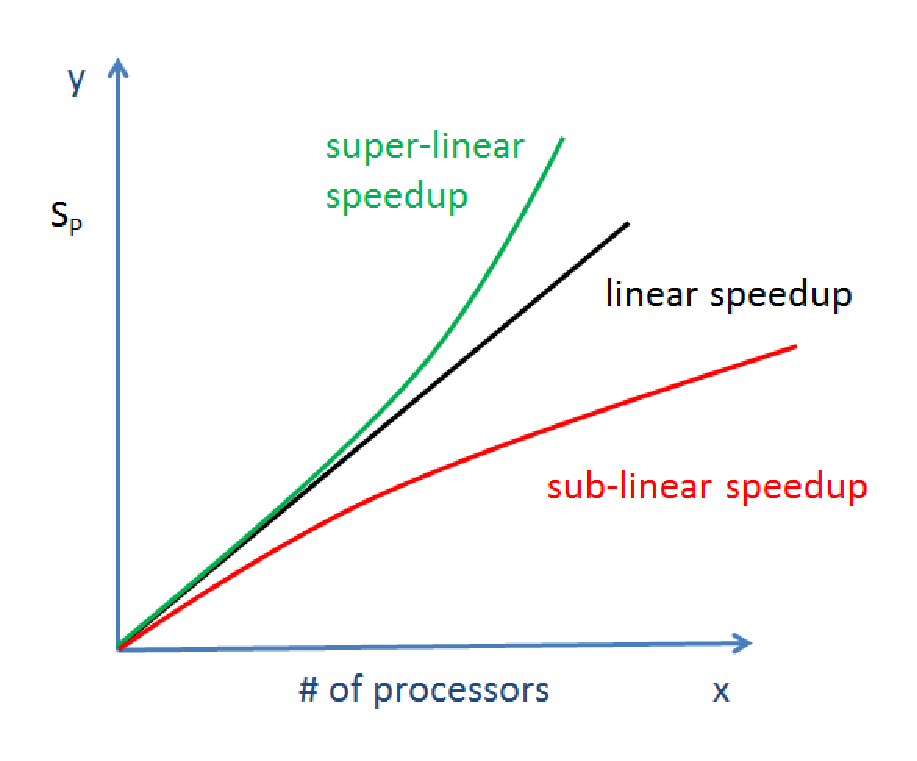
\includegraphics[scale=0.8]{TypesOfSpeedUp.pdf}
\caption{Speed-Up Types}
\label{fig:TypesOfSpeedUp}
\end{figure}

Efficiency is defined as a ratio of speed-up gained for \textit{N} processors to the number of processors. The Equation \ref{eq:eff} is used to calculate the efficiency.

\begin{equation}
\label{eq:eff}
\begin{aligned}
E_{N} = S_{N}/N
\end{aligned}
\end{equation}

\subsubsection{Distributed Cuttlefish Prototype I vs Non-Distributed Cuttlefish}

To check the speed-up gained by Distributed Cuttlefish Prototype I, the application was run with different work-loads and comparison between the execution times for both Distributed Cuttlefish Prototype I and Non-Distributed Cuttlefish application was drawn.

\begin{enumerate}
\item{\textbf{Scenario}}- To test the computational speed-up gained by distributed cuttlefish prototype I in comparison to non-distributed cuttlefish for input consisting of same models.
\begin{itemize}
\item{\textbf{Test-Case and Test-Data Description}}- The cluster was composed of 3 nodes where in one node was the master and remaining two were compute nodes. The cluster nodes were heterogeneous in terms of the number of cores, CPU speed and RAM capacity. The test-data included multiple head models of size 8cms. The number of head models was increased by 2 for each following test-case, i.e. starting with 2 head models the number was increased to 10 head models for the 5 test-cases, with each test-case executed 5 times to enable collection of the average execution times. The speed-up for each test case was calculated using the average execution time for distributed cuttlefish and non-distributed cuttlefish for a given test-data i.e. given work-load. The non-distributed cuttlefish application was executed on the slowest node of the cluster as the slowest node in the cluster would impact the execution time of the distributed version. 
\item{\textbf{Results}}- To elaborate on the amount of work to be done, each 8 cm head model consists of 777 slices with each slice having the width-946 voxels along X-axis (8.00 cm)and height-303 voxels along Y-axis(5.12 cm). The total number of voxels for each model is calculated using the Equation \ref{eq:NumVoxel} where, \begin{math} T_{NumVoxels} \end{math} is the total number of voxels for a given model, width (W), height(H) and total number of slices- NumSlices. For each head model used in the test data, the total number of voxels to be processed is \begin{math} 2.2 \times 10^{8} \end{math}. Each voxel can be assigned values denoting the materials and a null material value depending upon the printer specification provided. For current test case, the materials provided in the printer specification are VeroCyan, VeroWhite, VeroMagenta, VeroYellow, VeroBlack and EMPTY\_VOXEL as null material . For each material there is a bitmap generated denoting the voxels which are assigned that particular material in the slice. Figure \ref{fig:SliceOutput} shows the material assignment generated for 108th slice of a single head model. The Table \ref{protoIvsND} summarizes the execution times for distributed cuttlefish with prototype I and non-distributed cuttlefish along with the speed-up.  
\item{\textbf{Observation}}- The number of slave nodes is constant throughout the test-cases i.e. 2 slave nodes and the work-load provided to the system is increased for every test-case. The speed-up is calculated as per the Equation \ref{eq:speed-up} and it increases with the increase in work-load in comparison to the non-distributed cuttlefish performance. The red line in Figure \ref{fig:SUPIPIIvsNumMod} depicts the scaling of the speed-up with increase in work load i.e number of models. This is proved by calculating the efficiency using the Equation \ref{eq:eff} and seen in the Figure \ref{fig:EffPIPIIvsNumMod}. 
\end{itemize}

\item{\textbf{Scenario}}- To test the computational speed-up gained by distributed cuttlefish prototype I in comparison to non-distributed cuttlefish for input consisting of different models.
\begin{itemize}
\item{\textbf{Test-Case and Test-Data Description}}- The test case was executed 5 times for each test-data. The cluster was composed of 3 nodes where in one node was the master and remaining two were compute nodes. The cluster nodes were heterogeneous in terms of the number of cores, CPU speed and RAM capacity. The test-data included multiple head and dame models of size 8 cm. The number of models was increased by 2 for each following test-case, i.e. starting with 1 head model and 1 dame model, the number was increased to 5 head and dame models each, for the 5 test-cases, with each test-case executed 5 times to enable collection of the average execution times. The speed-up for each test case was calculated using the average execution time for distributed cuttlefish and non-distributed cuttlefish for a given test-data i.e. given work-load. The non-distributed cuttlefish application was executed on the slowest node of the cluster as the slowest node in the cluster would impact the execution time of the distributed version. 
\item{\textbf{Results}}- To elaborate on the amount of work to be done, each 8cms head model consists of 777 slices, with each slice having the width-946 voxels along X-axis (8.00 cm)and height-303 voxels along Y-axis (5.12 cm). The total number of voxels for each model is calculated using the following Equation \ref{eq:NumVoxel} where, \begin{math} T_{NumVoxels} \end{math} is the total number of voxels for a given model, width (W), height(H) and and total number of slices- NumSlices. For each head model used in the test data, the total number of voxels to be processed is \begin{math} 2.2 \times 10^{8} \end{math}. Each 8cm dame model consists of 605 slices, with each slice having the width-946 voxels along X-axis (8.00 cm)and height-194 voxels along Y-axis (3.27035 cm). The total number of voxels for the dame model calculated using the Equation \ref{eq:NumVoxel} is  \begin{math} 1.1 \times 10^{8} \end{math}. Each voxel can be assigned values denoting the materials and a null material value depending upon the printer specification provided. For current test case, the materials provided in the printer specification are VeroCyan, VeroWhite, VeroMagenta, VeroYellow, VeroBlack and EMPTY\_VOXEL as null material . For each material there is a bitmap generated denoting the voxels which are assigned that particular material in the slice. The Table \ref{protoIvsNDDiffModel} summarizes the execution times for distributed cuttlefish with prototype I and non-distributed cuttlefish along with the speed-up for input consisting of different models.  
\item{\textbf{Observation}}-  The number of slave nodes is constant throughout the test-cases i.e. 2 slave nodes and the work-load provided to the system is increased for every test-case. The speed-up is calculated as per the Equation \ref{eq:speed-up} and increases with the increase in work-load in comparison to the non-distributed cuttlefish performance. The red line in the Figure \ref{fig:SUPIPIIvsNumModDM},  depicts that Prototype I speed-up increases with increase in work load i.e number of models. This is proved by calculating the efficiency using the Equation \ref{eq:eff} and plot seen in the Figure \ref{fig:EffPIPIIvsNumModDM}. 
\end{itemize}
\end{enumerate}

\begin{table}
\centering
\caption{Speed-Up and Efficiency: Distributed Cuttlefish Prototype I vs Non-Distributed Cuttlefish For Same Models}
\label{protoIvsND}
\begin{tabular}{|c|l|l|l|c|}
\hline
\textbf{\begin{tabular}[c]{@{}c@{}}Number of \\ Head Models\\ 8cms\\ (Resolution:\\ 300 X 150 X 470)\end{tabular}} & \multicolumn{1}{c|}{\textbf{\begin{tabular}[c]{@{}c@{}}Total Execution Time (in Secs)\\  for Distributed \\ Cuttlefish Prototype I\\ (Cluster Size- 3)\end{tabular}}} & \multicolumn{1}{c|}{\textbf{\begin{tabular}[c]{@{}c@{}}Total Execution Time (in Secs) \\ for Non-Distributed\\ Cuttlefish\end{tabular}}} & \multicolumn{1}{c|}{\textbf{Speed-Up}} & \textbf{Efficiency} \\ \hline
2                                                                                                                  & 173.35                                                                                                                                                    & 357.35                                                                                                                       & 2.06                              & 0.68           \\ \hline
4                                                                                                                  & 363.39                                                                                                                                                    & 920.56                                                                                                                        & 2.53                              & 0.84          \\ \hline
6                                                                                                                  & 585.32                                                                                                                                                    & 1651.17                                                                                                                      & 2.82                            & 0.94           \\ \hline
8                                                                                                                  & 836.23                                                                                                                                                    & 4071.57                                                                                                                       & 4.86                              & 1.62           \\ \hline
10                                                                                                                 & 1130.51                                                                                                                                                    & 4790.19                                                                                                                       & 4.23                              & 1.41          \\ \hline
\end{tabular}
\end{table}


\begin{table}
\centering
\caption{Speed-Up and Efficiency: Distributed Cuttlefish Prototype I vs Non-Distributed Cuttlefish For Different Models}
\label{protoIvsNDDiffModel}
\begin{tabular}{|c|l|l|l|c|}
\hline
\textbf{\begin{tabular}[c]{@{}c@{}}Number of \\ Head \& Dame\\  Models -8 cm\\ (Resolution:\\ 300 X 150 X 470)\end{tabular}} & \multicolumn{1}{c|}{\textbf{\begin{tabular}[c]{@{}c@{}}Total Execution Time \\ (in secs)\\  for Distributed \\ Cuttlefish Prototype I\\ (Cluster Size- 3)\end{tabular}}} & \multicolumn{1}{c|}{\textbf{\begin{tabular}[c]{@{}c@{}}Total Execution Time\\ (in secs) \\ for Non-Distributed\\ Cuttlefish\end{tabular}}} & \multicolumn{1}{c|}{\textbf{Speed-Up}} & \textbf{Efficiency} \\ \hline
2                                                                                                                            & 184.25                                                                                                                                                                   & 243.94                                                                                                                                     & 1.32                            & 0.44        \\ \hline
4                                                                                                                            & 315.34                                                                                                                                                                  & 635.52                                                                                                                                    & 2.01                            & 0.67         \\ \hline
6                                                                                                                            & 563.3                                                                                                                                                                    & 1171.32                                                                                                                                    & 2.07                            & 0.69         \\ \hline
8                                                                                                                            & 685.21                                                                                                                                                                   & 1890.70                                                                                                                                   & 2.75                            & 0.91         \\ \hline
10                                                                                                                           & 988.70                                                                                                                                                                  & 4793.47                                                                                                                                    & 4.84                            & 1.61         \\ \hline
\end{tabular}
\end{table}

\begin{figure}[t]
\centering
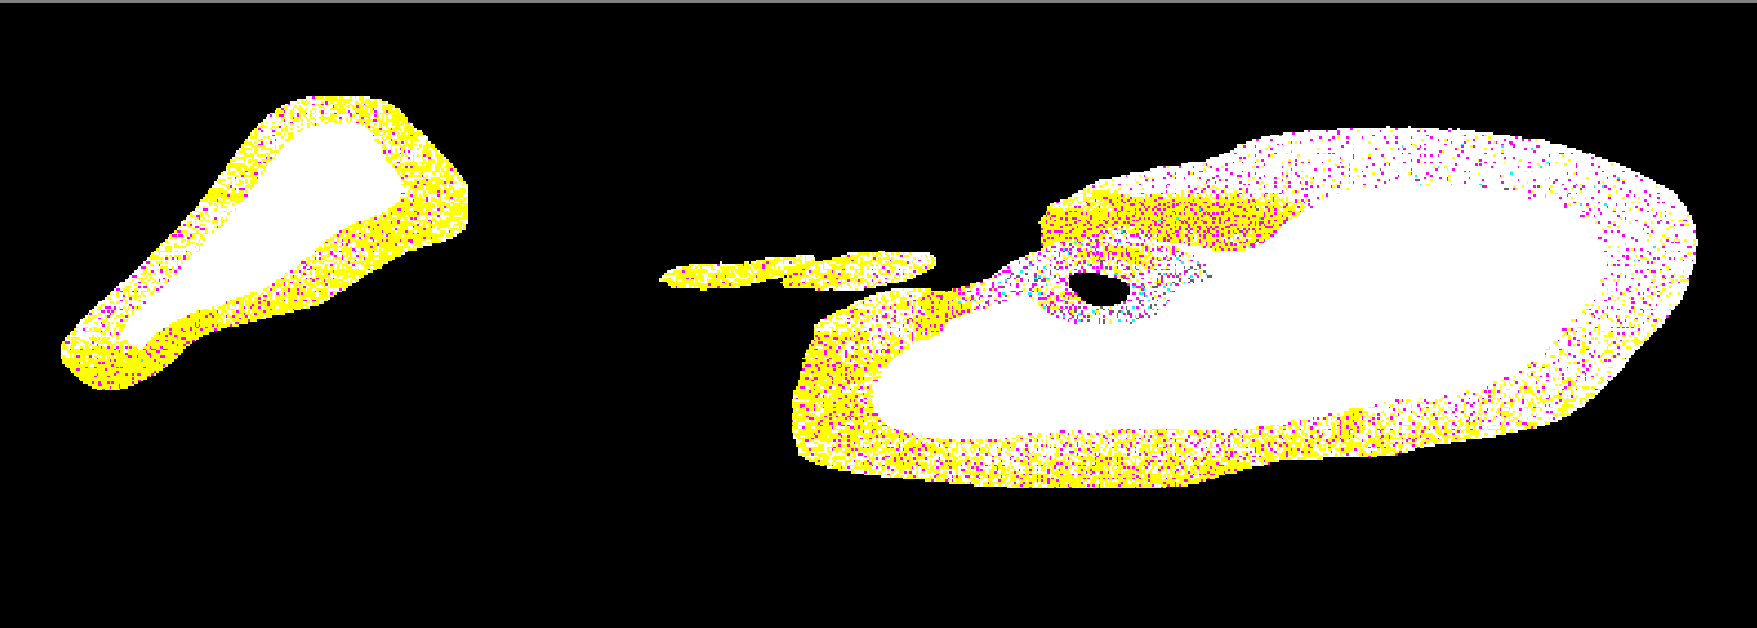
\includegraphics[scale=0.5]{SliceOutput.pdf}
\caption{Material Assignment for Single Slice}
\label{fig:SliceOutput}
\end{figure}

\begin{figure}
\centering
\begin{subfigure}
\centering
\captionsetup[subfigure]{labelformat=empty}
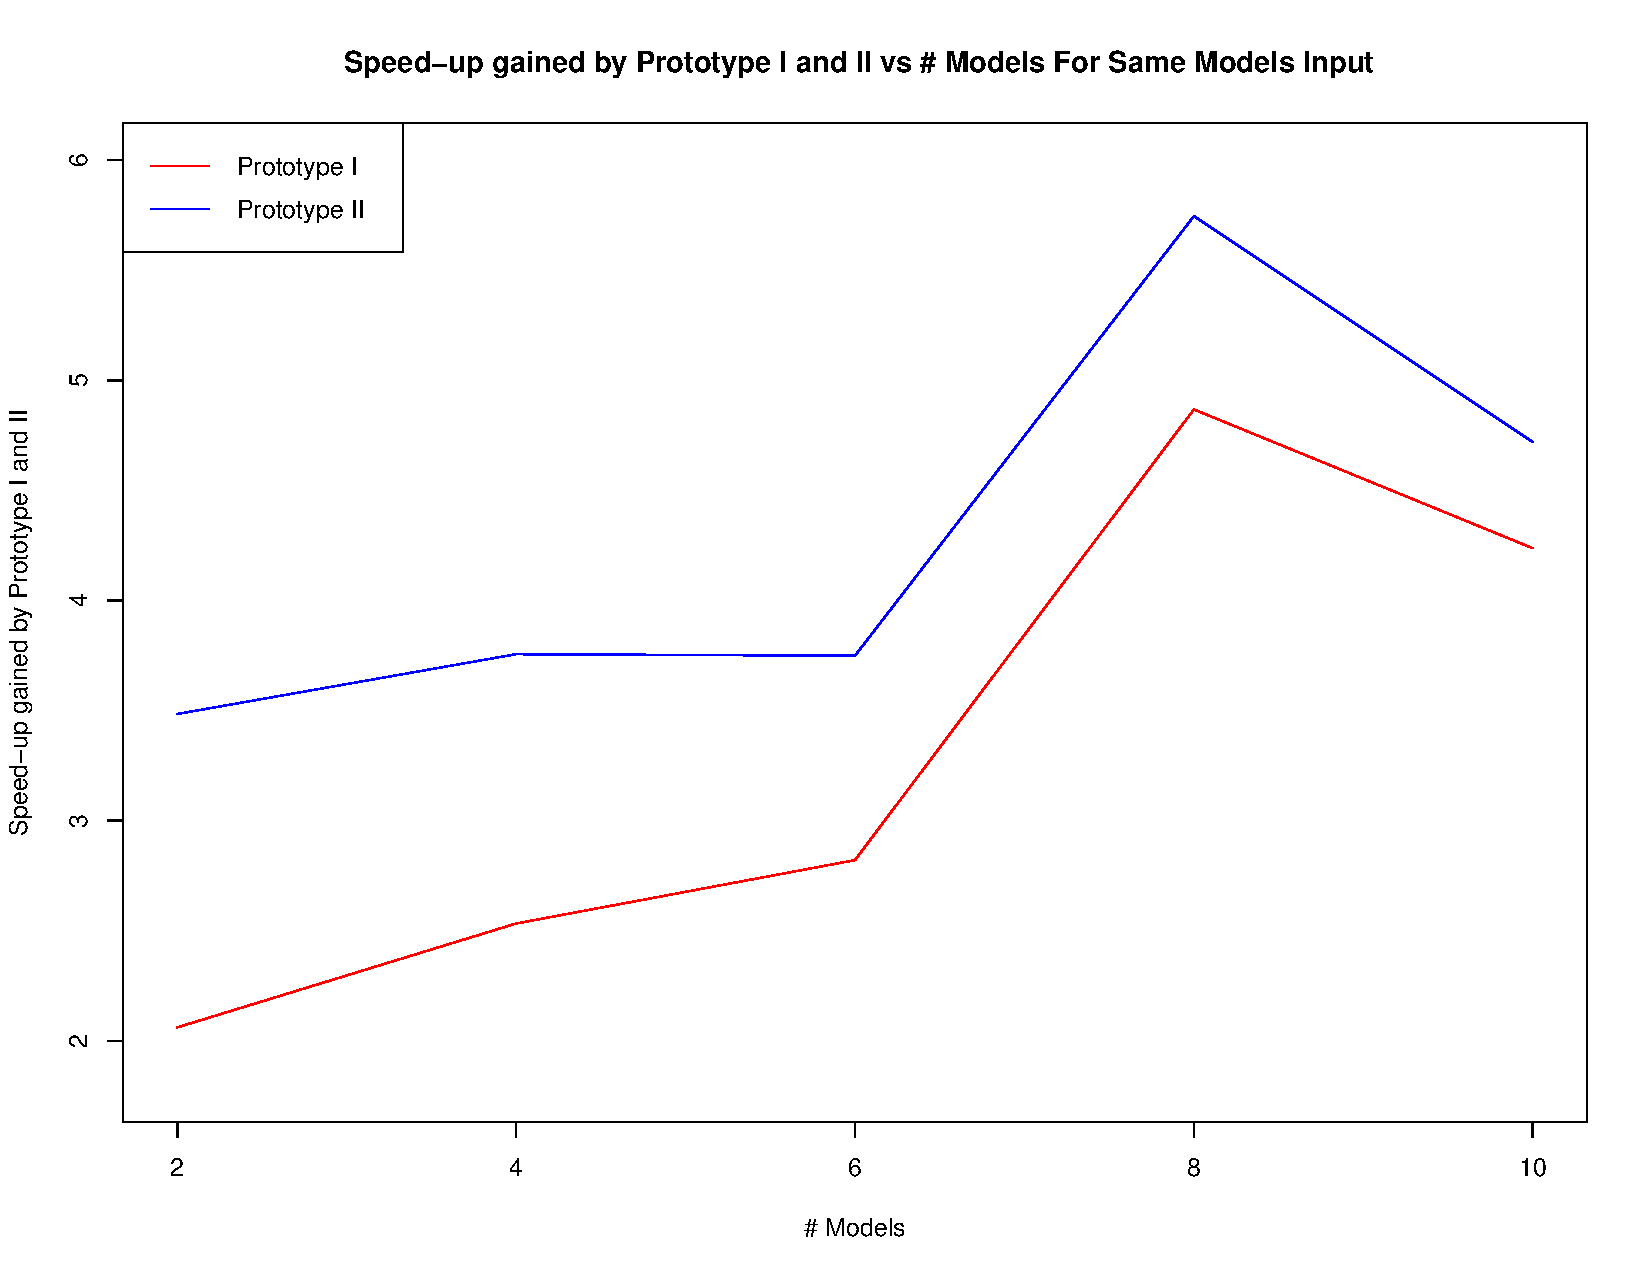
\includegraphics[scale=0.5]{SUPIPIIvsNumMod.pdf}
\caption{Speed-up Vs Number of Models For Same Models Input}
\label{fig:SUPIPIIvsNumMod}
\end{subfigure}
\begin{subfigure}
\centering
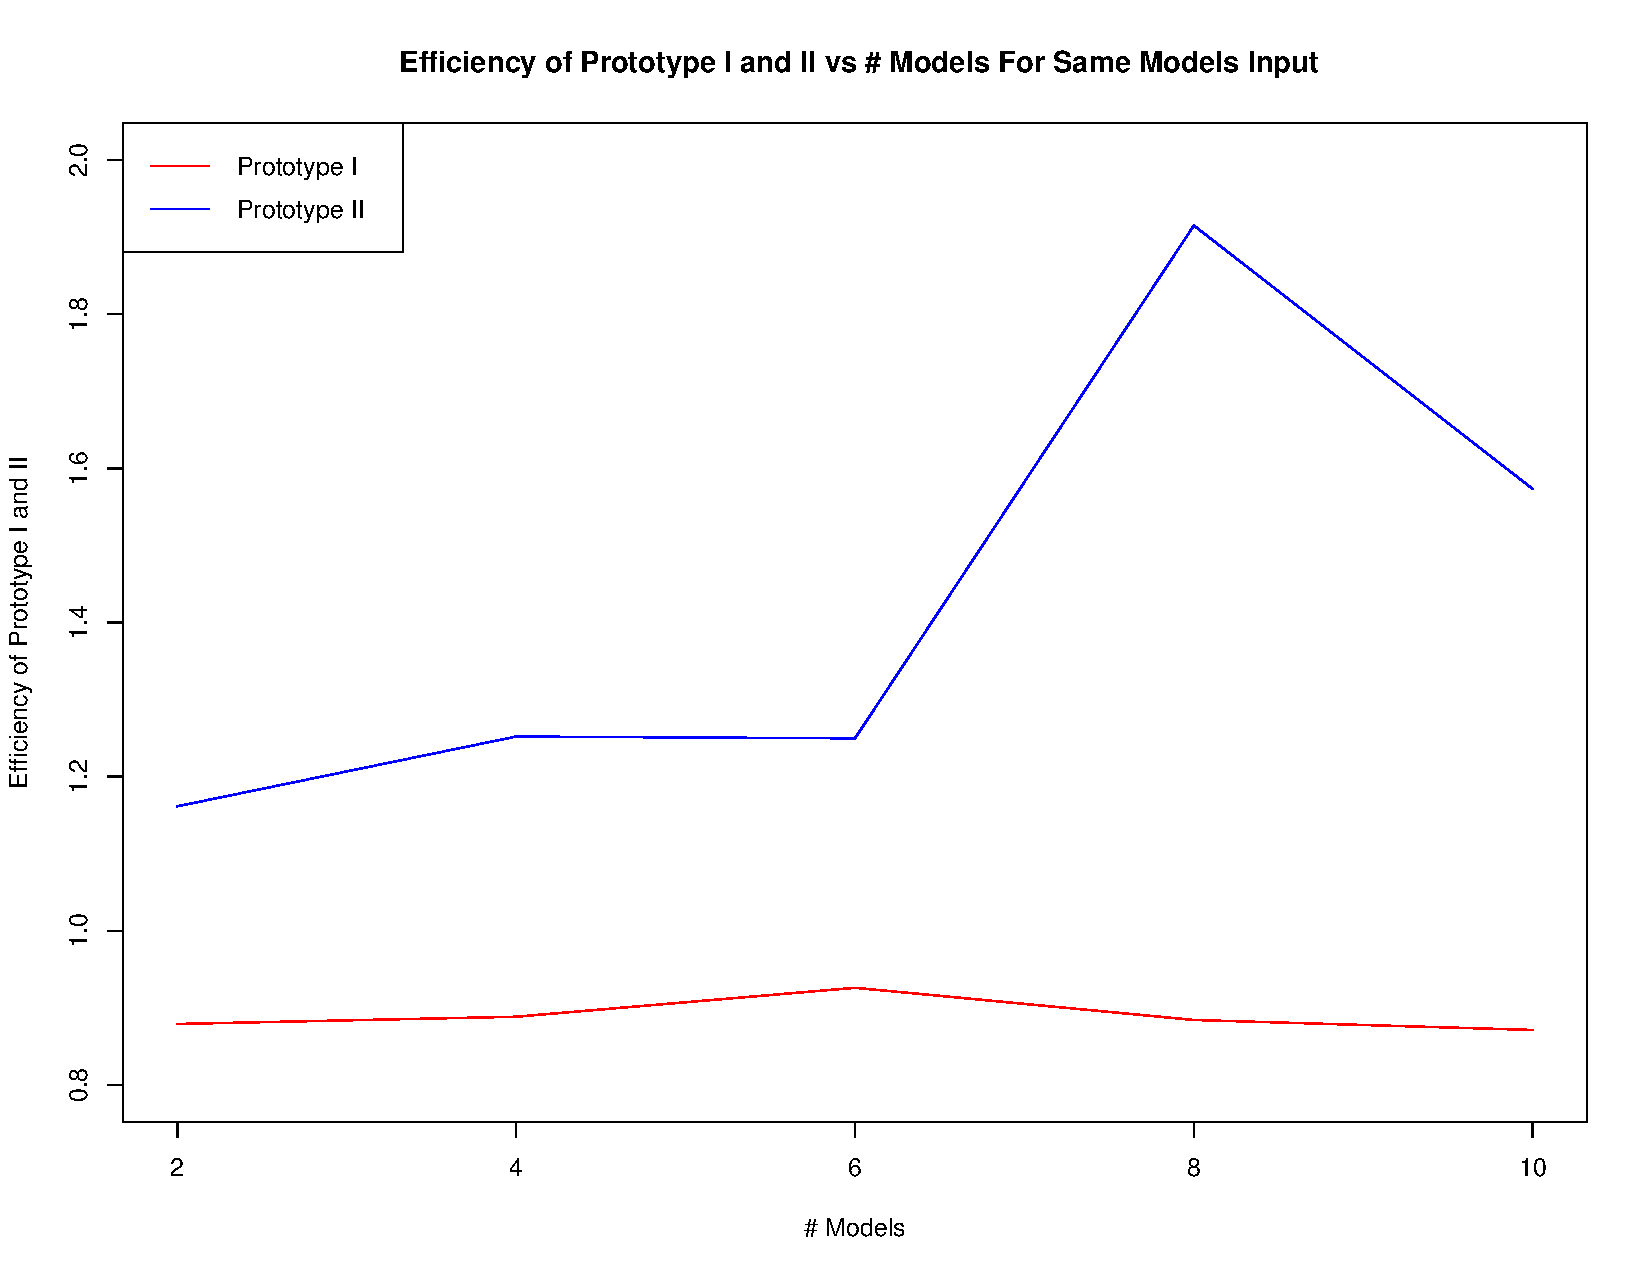
\includegraphics[scale=0.5]{EffPIPIIvsNumMod.pdf}
\caption{Efficiency Vs Number of Models For Same Models Input}
\label{fig:EffPIPIIvsNumMod}
\end{subfigure}
\end{figure}


\begin{figure}
\centering
\captionsetup[subfigure]{labelformat=empty}
\begin{subfigure}
\centering
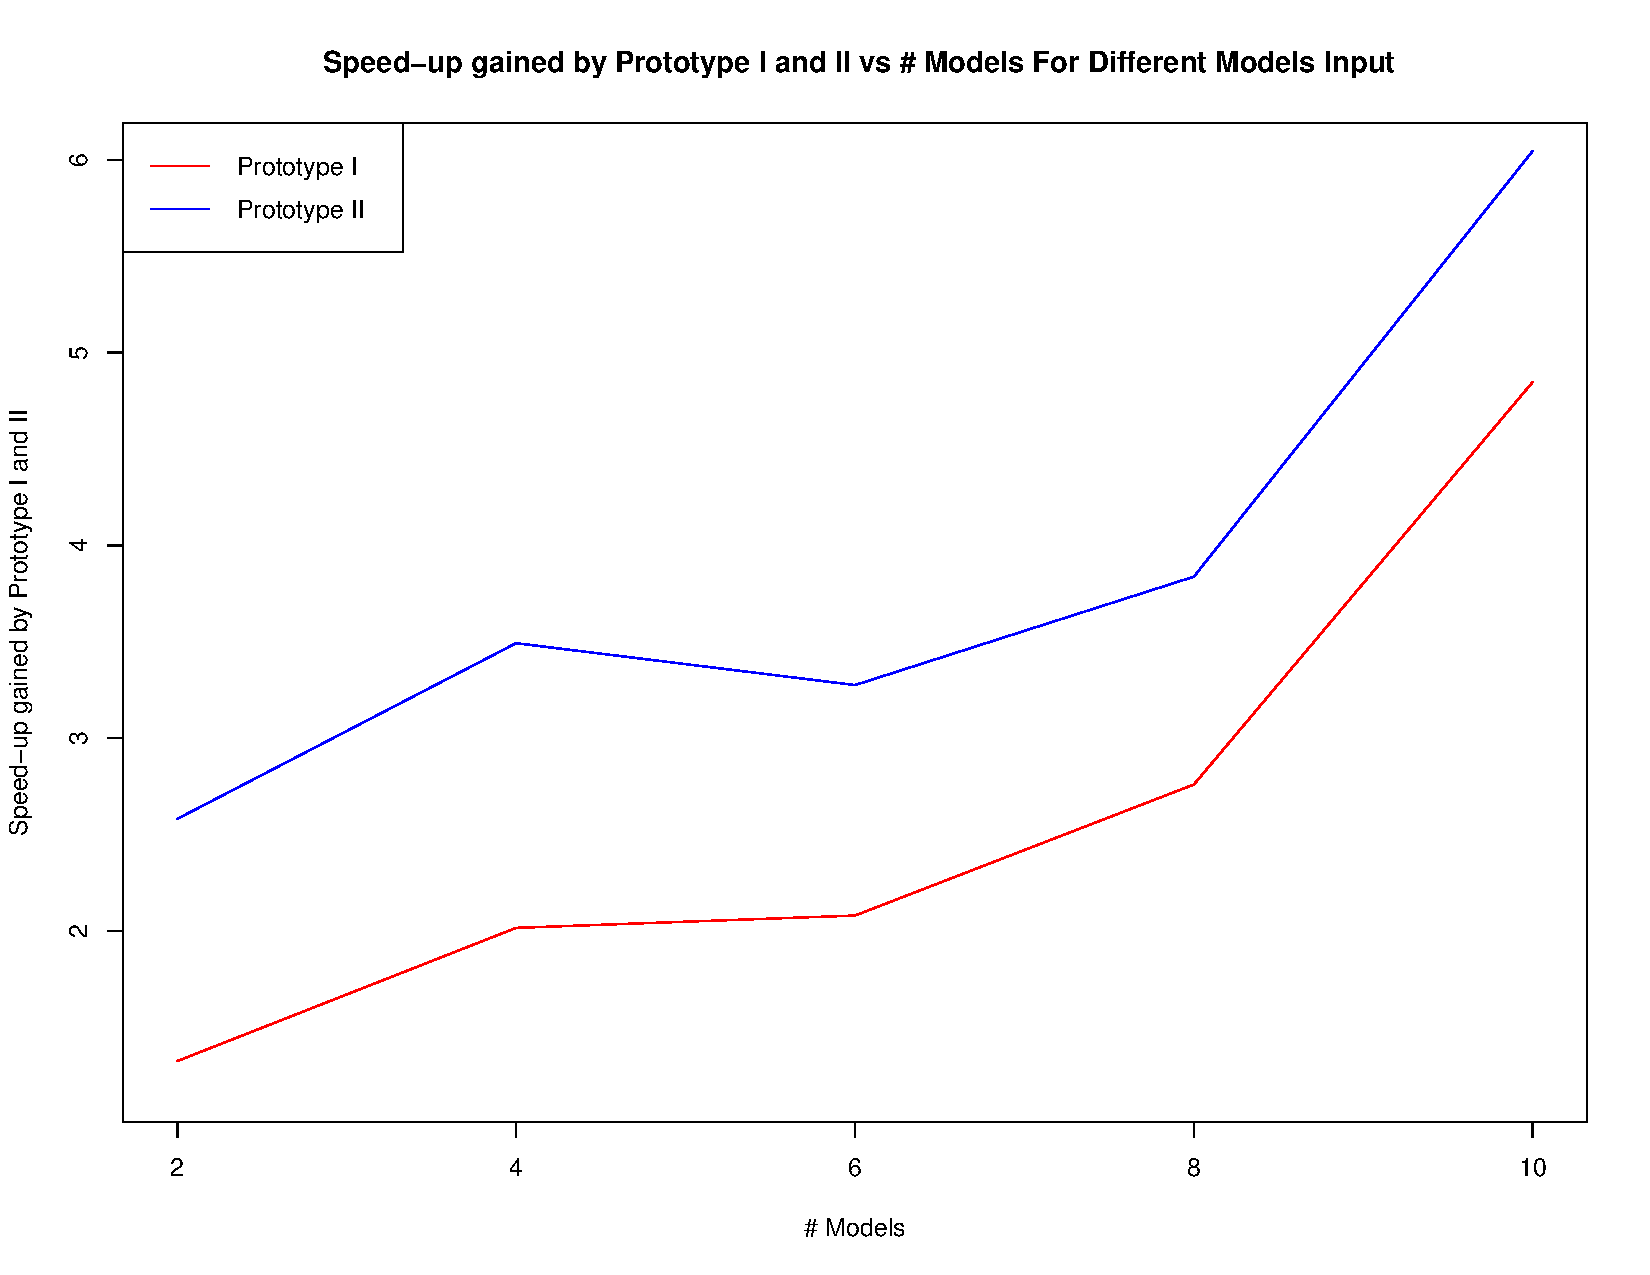
\includegraphics[scale=0.5]{SUPIPIIvsNumModDM.pdf}
\caption{Speed-up Vs Number of Models For Different Models Input}
\label{fig:SUPIPIIvsNumModDM}
\end{subfigure}
\begin{subfigure}
\centering
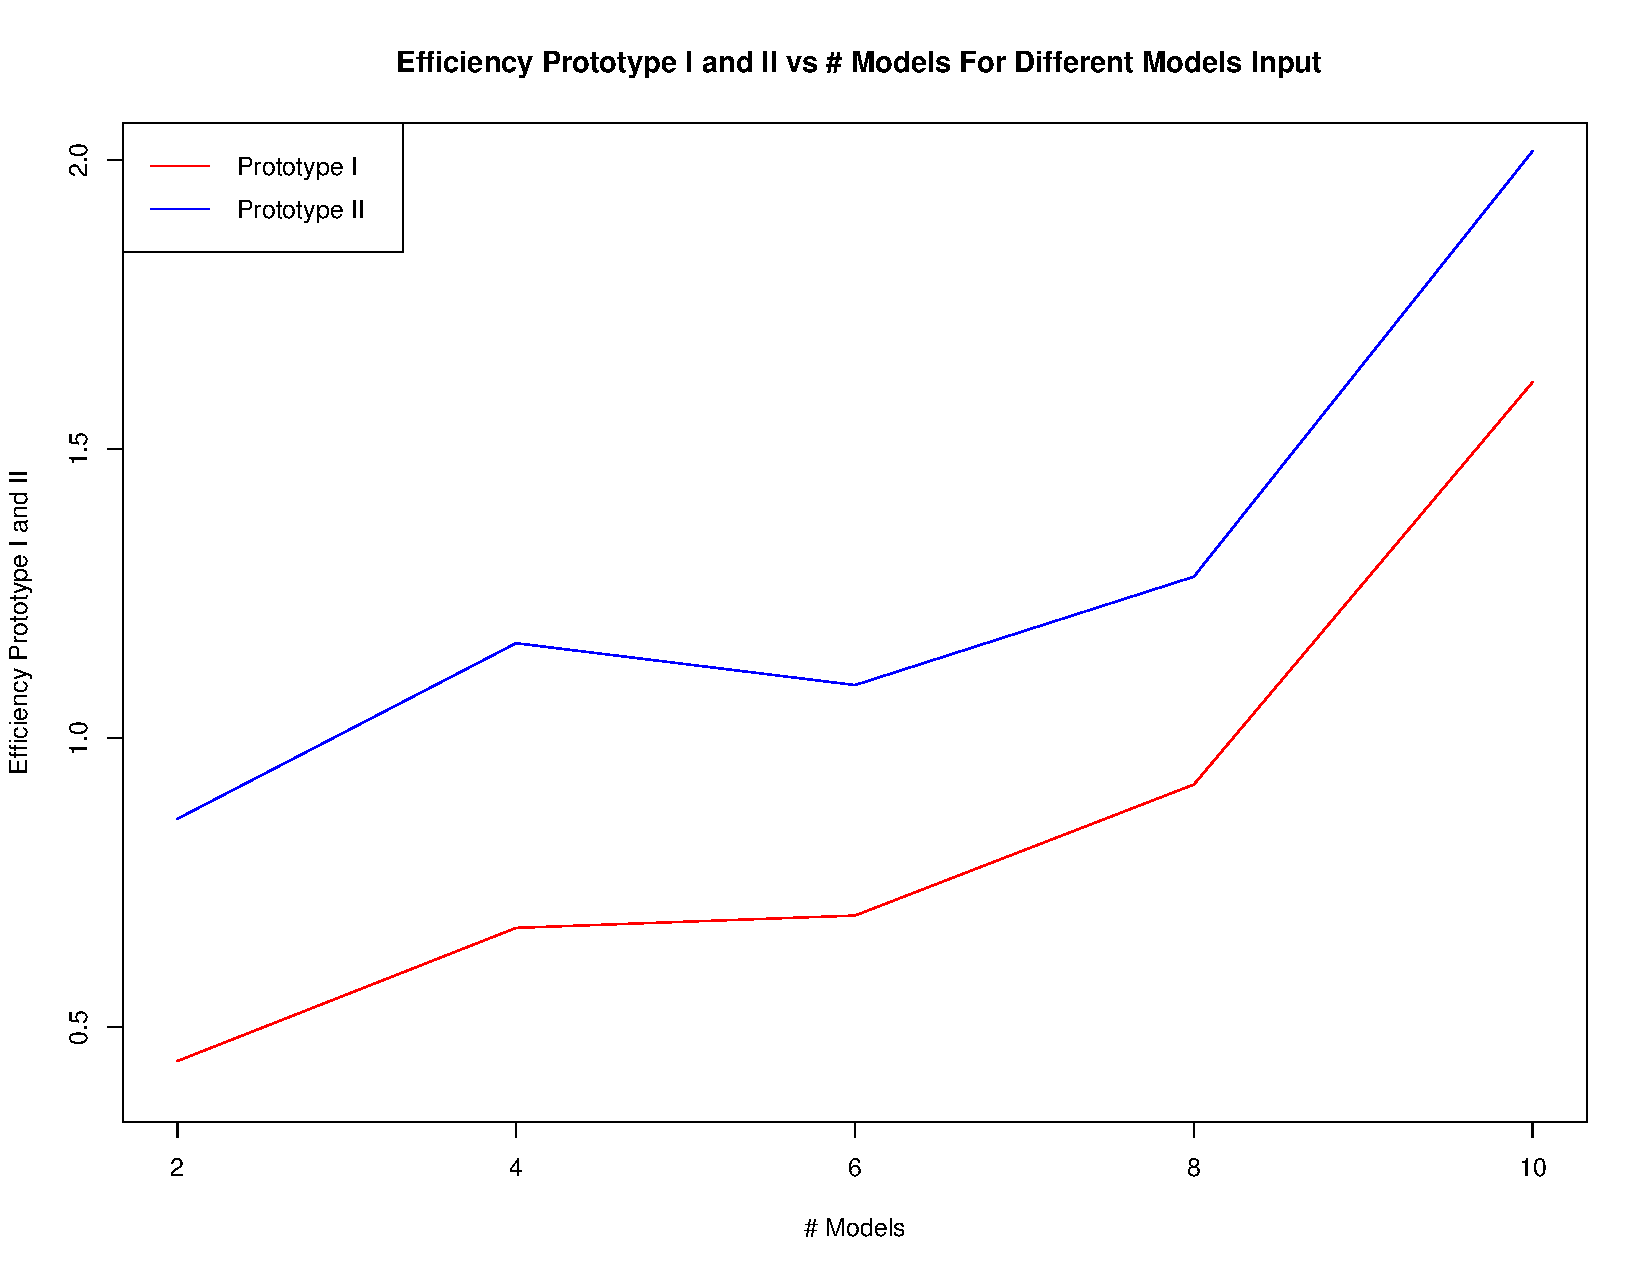
\includegraphics[scale=0.5]{EffPIPIIvsNumModDM.pdf}
\caption{Efficiency Vs Number of Models For Different Models Input}
\label{fig:EffPIPIIvsNumModDM}
\end{subfigure}
\end{figure}


\begin{equation}
\label{eq:NumVoxel}
\begin{aligned}
T_{NumVoxels} = W \times H \times NumSlices
\end{aligned}
\end{equation}


\subsubsection{Distributed Cuttlefish Prototype II vs Non-Distributed Cuttlefish}
To check the speed-up gained by using the Distributed Cuttlefish Prototype II, the application was run with different work-loads and comparison between the execution times for both Distributed Cuttlefish Prototype I and Non-Distributed Cuttlefish application was drawn.

\begin{enumerate}
\item{\textbf{Scenario}}- To test the computational speed-up gained by distributed cuttlefish prototype II in comparison to non-distributed cuttlefish for input consisting of same models.
\begin{itemize}
\item{\textbf{Test-Case and Test-Data Description}}- The test-case and the test-data used here is exactly same as the test-case and test-data of Scenario 1 of Prototype I.
\item{\textbf{Results}}- The amount of work done by the nodes remains same as described in Scenario 1 of Prototype I testing. The Table \ref{ProtoIISameModelsVsND} summarizes the execution time for the test case for prototype II.
\item{\textbf{Observation}}- The speed-up for the prototype II was calculated using the Equation \ref{eq:speed-up} and efficiency was calculated using the Equation \ref{eq:eff}. The blue line in the Figure \ref{fig:SUPIPIIvsNumMod} and Figure \ref{fig:EffPIPIIvsNumMod} depict the trend seen for the speed-up and efficiency for prototype II. As the number of models increases the speed-up and efficiency increases for a given cluster size until a certain point (i.e. until the number of models reaches 8 models, at which there is peak performance seen) after which with increase in number of models the speed-up decreases and so does the efficiency.  
\end{itemize}

\item{\textbf{Scenario}}- To test the computational speed-up gained by distributed cuttlefish prototype II in comparison to non-distributed cuttlefish for input consisting of different models.
\begin{itemize}
\item{\textbf{Test-Case and Test-Data Description}}- The test-case and the test-data used here is exactly same as the test-case and test-data of Scenario 2 of Prototype I.
\item{\textbf{Results}}- The amount of work done by the nodes remains same as described in Scenario 2 of Prototype I testing. The Table \ref{ProtoIIDiffModelsVsND} summarizes the execution time for the test case for prototype II.
\item{\textbf{Observation}}-  The speed-up for the prototype II was calculated using the Equation \ref{eq:speed-up} and efficiency was calculated using the Equation \ref{eq:eff}. The blue line in the Figure \ref{fig:SUPIPIIvsNumModDM} and Figure \ref{fig:EffPIPIIvsNumModDM} depict the trend seen for the speed-up and efficiency for prototype II for different models as input set. As the number of models increases the speed-up and efficiency increases.
\end{itemize}
\end{enumerate}


\begin{table}
\centering
\caption{Speed-Up and Efficiency: Distributed Cuttlefish Prototype II vs Non-Distributed Cuttlefish for Same Models}
\label{ProtoIISameModelsVsND}
\begin{tabular}{|c|l|l|l|c|}
\hline
\textbf{\begin{tabular}[c]{@{}c@{}}Number of \\ Head -8 cm\\ (Resolution:\\ 300 X 150 X 470)\end{tabular}} & \multicolumn{1}{c|}{\textbf{\begin{tabular}[c]{@{}c@{}}Total Execution Time \\ (in secs)\\  for Distributed \\ Cuttlefish Prototype II\\ (Cluster Size- 3)\end{tabular}}} & \multicolumn{1}{c|}{\textbf{\begin{tabular}[c]{@{}c@{}}Total Execution Time\\ (in secs) \\ for Non-Distributed\\ Cuttlefish\end{tabular}}} & \multicolumn{1}{c|}{\textbf{Speed-Up}} & \textbf{Efficiency} \\ \hline
2                                                                                                          & 102.55                                                                                                                                                                  & 357.35                                                                                                                                    & 3.48                            & 1.16         \\ \hline
4                                                                                                          & 245.08                                                                                                                                                                  & 920.56                                                                                                                                    & 3.75                            & 1.25         \\ \hline
6                                                                                                          & 440.41                                                                                                                                                                   & 1651.17                                                                                                                                   & 3.74                            & 1.24         \\ \hline
8                                                                                                          & 708.70                                                                                                                                                                   & 4071.56                                                                                                                                    & 5.74                            & 1.91        \\ \hline
10                                                                                                         & 1014.98                                                                                                                                                                 & 4790.19                                                                                                                                  & 4.71                            & 1.57         \\ \hline
\end{tabular}
\end{table}

\begin{table}
\centering
\caption{Speed-Up and Efficiency: Distributed Cuttlefish Prototype II vs Non-Distributed Cuttlefish for Different Models}
\label{ProtoIIDiffModelsVsND}
\begin{tabular}{|c|c|c|c|c|}
\hline
\textbf{\begin{tabular}[c]{@{}c@{}}Number of \\ Head \& Dame,\\ Models -8 cm\\ (Resolution:\\ 300 X 150 X 470)\end{tabular}} & \textbf{\begin{tabular}[c]{@{}c@{}}Total Execution Time \\  (in secs) for \\ Distributed \\ Cuttlefish Prototype II\\ (Cluster Size- 3)\end{tabular}} & \textbf{\begin{tabular}[c]{@{}c@{}}Total Execution Time\\ (in secs) for \\ Non-Distributed\\ Cuttlefish\end{tabular}} & \textbf{Speed-up} & \textbf{Efficiency-ProtoII} \\ \hline
2                                                                                                                            & 94.52                                                                                                                                              & 243.94                                                                                                                & 2.582       & 0.86                \\ \hline
4                                                                                                                            & 181.95                                                                                                                                              & 635.52                                                                                                               & 3.49       & 1.16                 \\ \hline
6                                                                                                                            & 357.61                                                                                                                                               & 1171.32                                                                                                               & 3.27       & 1.09                 \\ \hline
8                                                                                                                            & 492.65                                                                                                                                              & 1890.70                                                                                                              & 3.83       & 1.27                 \\ \hline
10                                                                                                                           & 792.68                                                                                                                                              & 4793.47                                                                                                               & 6.04       & 2.01                 \\ \hline
\end{tabular}
\end{table}


\subsubsection{Performance Analysis}

Distributed cuttlefish has super-linear speed-up in most of the tested cases in comparison to non-distributed cuttlefish. One of the most fundamental reasons is availability of more resources in terms of computational capacity and memory. The time required to perform same the task in distributed fashion is lesser than the non-distributed cuttlefish because the sub-tasks are computed in parallel allowing more work to be done in less time. The overhead of distribution of sub-tasks and collection of the partial results is negligible in comparison to the time to taken perform the same task on single machine with non-distributed cuttlefish. The division of one single task to sub-tasks decreases the amount of work-load  i.e. less number of print objects per compute node. Lesser number of print objects per compute node leads to smaller amount of data processing per node which helps to accelerate the performance due higher cache hit rates with smaller data. Smaller amount of data can be kept in main memory throughout the computation without having a significant impact of paging on the performance. With non-distributed cuttlefish, it has been observed that running the application with single models multiple times leads to better performance than running the application once with multiple models \cite{perComm}, thus supporting the hypothesis of smaller data leading to higher cache hits resulting in better performance. \newline

The implementation of the components handling the distributed computing specific tasks has been done in such a way that the processing of these tasks happens in parallel with the main executing thread and the worker threads block only when they await for some input. At the slave node, the \textit{SlaveReporter} component has two threads of execution wherein one thread is the main thread which performs chunk-wise processing of the input i.e. runs the pipeline components as the streaming architecture and the worker thread which is dedicated to perform the distributed computing specific tasks such as serialization, communication of data and meta-data and additionally compression in case of Prototype II. The worker thread blocks only when the buffer of holding the partial slices is empty. The design of \textit{SlaveReporter} component is discussed in detail in the Section \ref{SRepoComp}. This design allows for minimum blocking time between the main thread and worker thread leading parallel computation and masks the latency that might be induced due to the communication between master and slave nodes. At the master node, the \textit{MasterMerger} component main thread creates a worker thread per slave which interacts with the worker thread from the slave node. This allows for communication between master node and slave nodes in parallel without the slaves blocking for one another. Also at the master nodes, the main thread can proceed with rest of the pipeline components when the container is ready with a minimum number of merged slices. The design of the \textit{MasterMerger} component is discussed in detail in the Section \ref{MMComp}. Due to this design, the overhead related to communication, deserialization, decompression is comparatively low. \newline
 

\subsection{Comparison of Distributed Cuttlefish Prototypes} \label{ProtoComp}

After comparing the performance of distributed cuttlefish vs non-distributed cuttlefish, to understand the performance of the prototypes in comparison with each other some tests were done. The aim of the tests was to understand how well the prototypes scale by varying cluster size for a given workload. The underlying assumption is that for a given workload, if the number of slave nodes in the cluster increases, the speed-up should also increase thus increasing the efficiency of the prototype. 

\begin{figure}
\centering
\captionsetup[subfigure]{labelformat=empty}
\begin{subfigure}
\centering
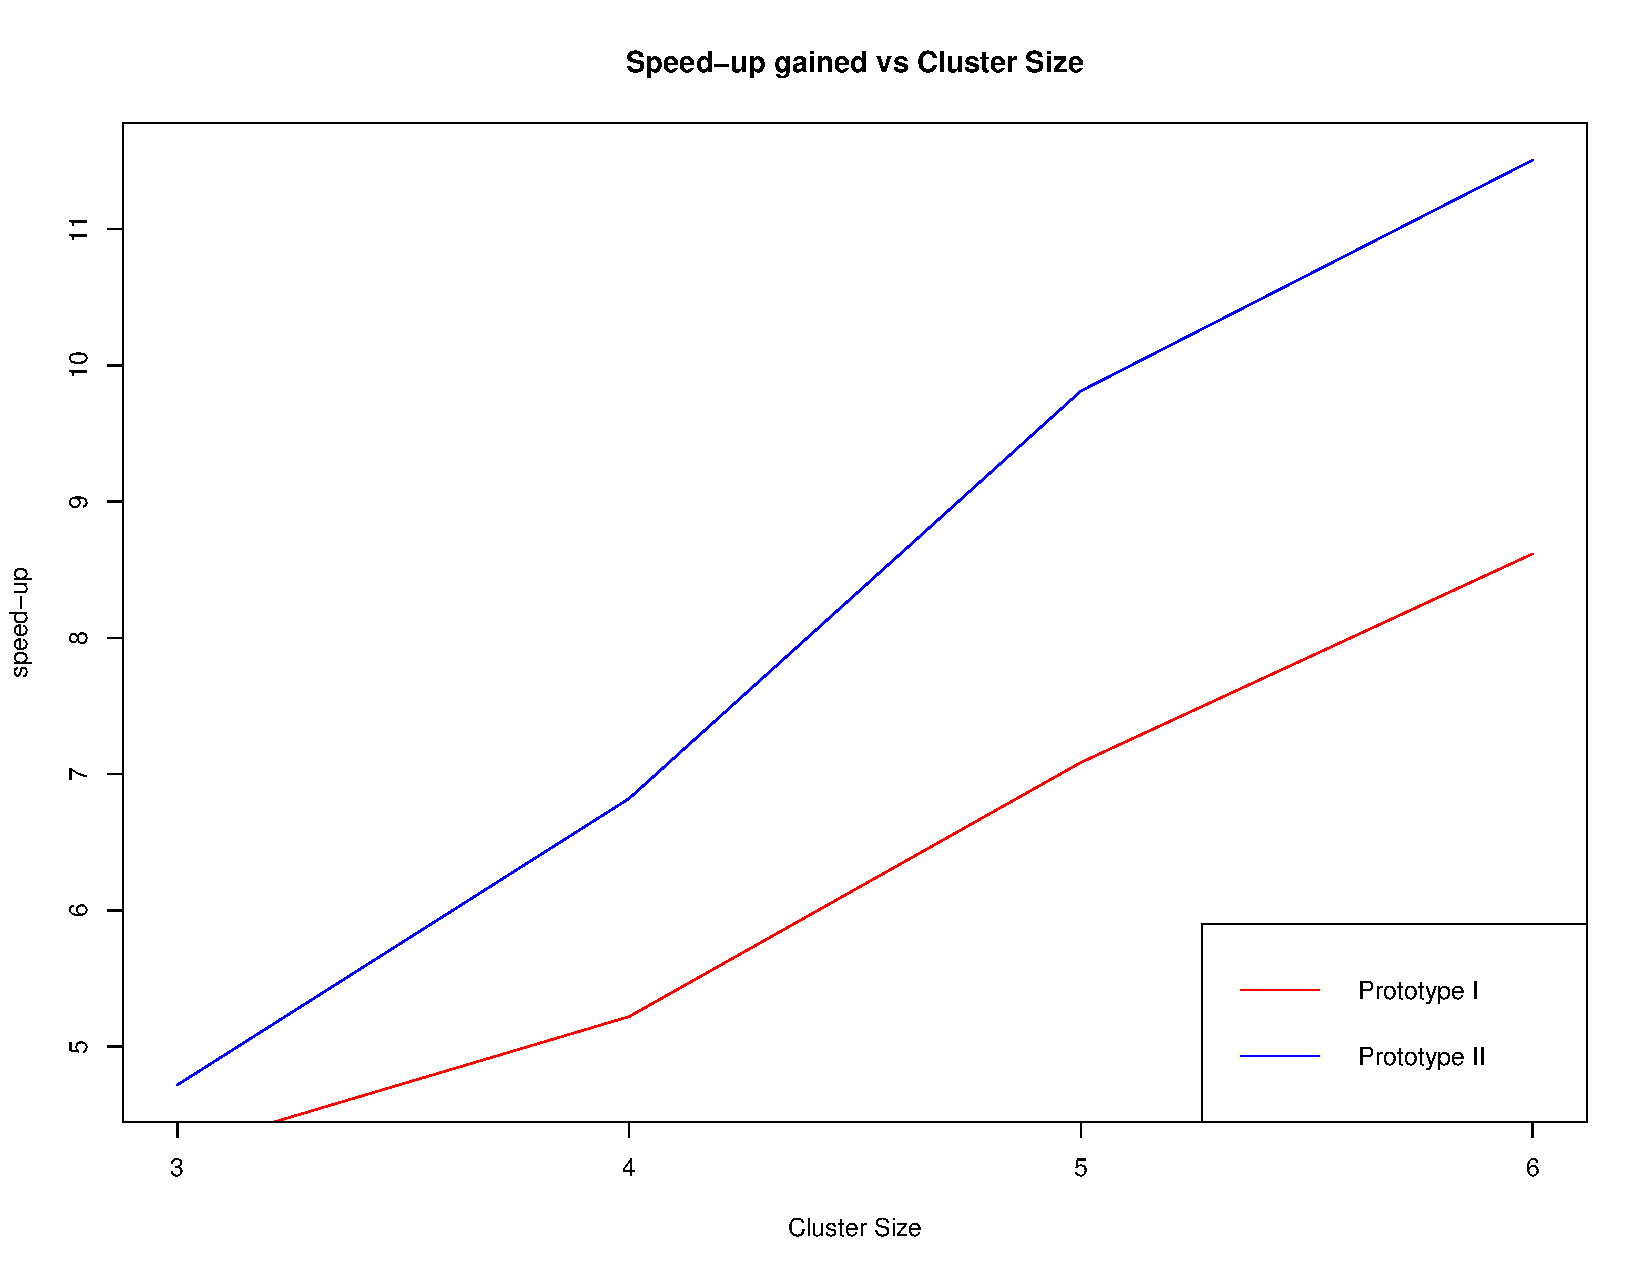
\includegraphics[scale=0.5]{SpeedupProtoIvsPrototII.pdf}
\caption{Speed-up of Prototype I and II Vs Cluster Size For Same Models Input Set}
\label{fig:SUPIPII}
\end{subfigure}
\begin{subfigure}
\centering
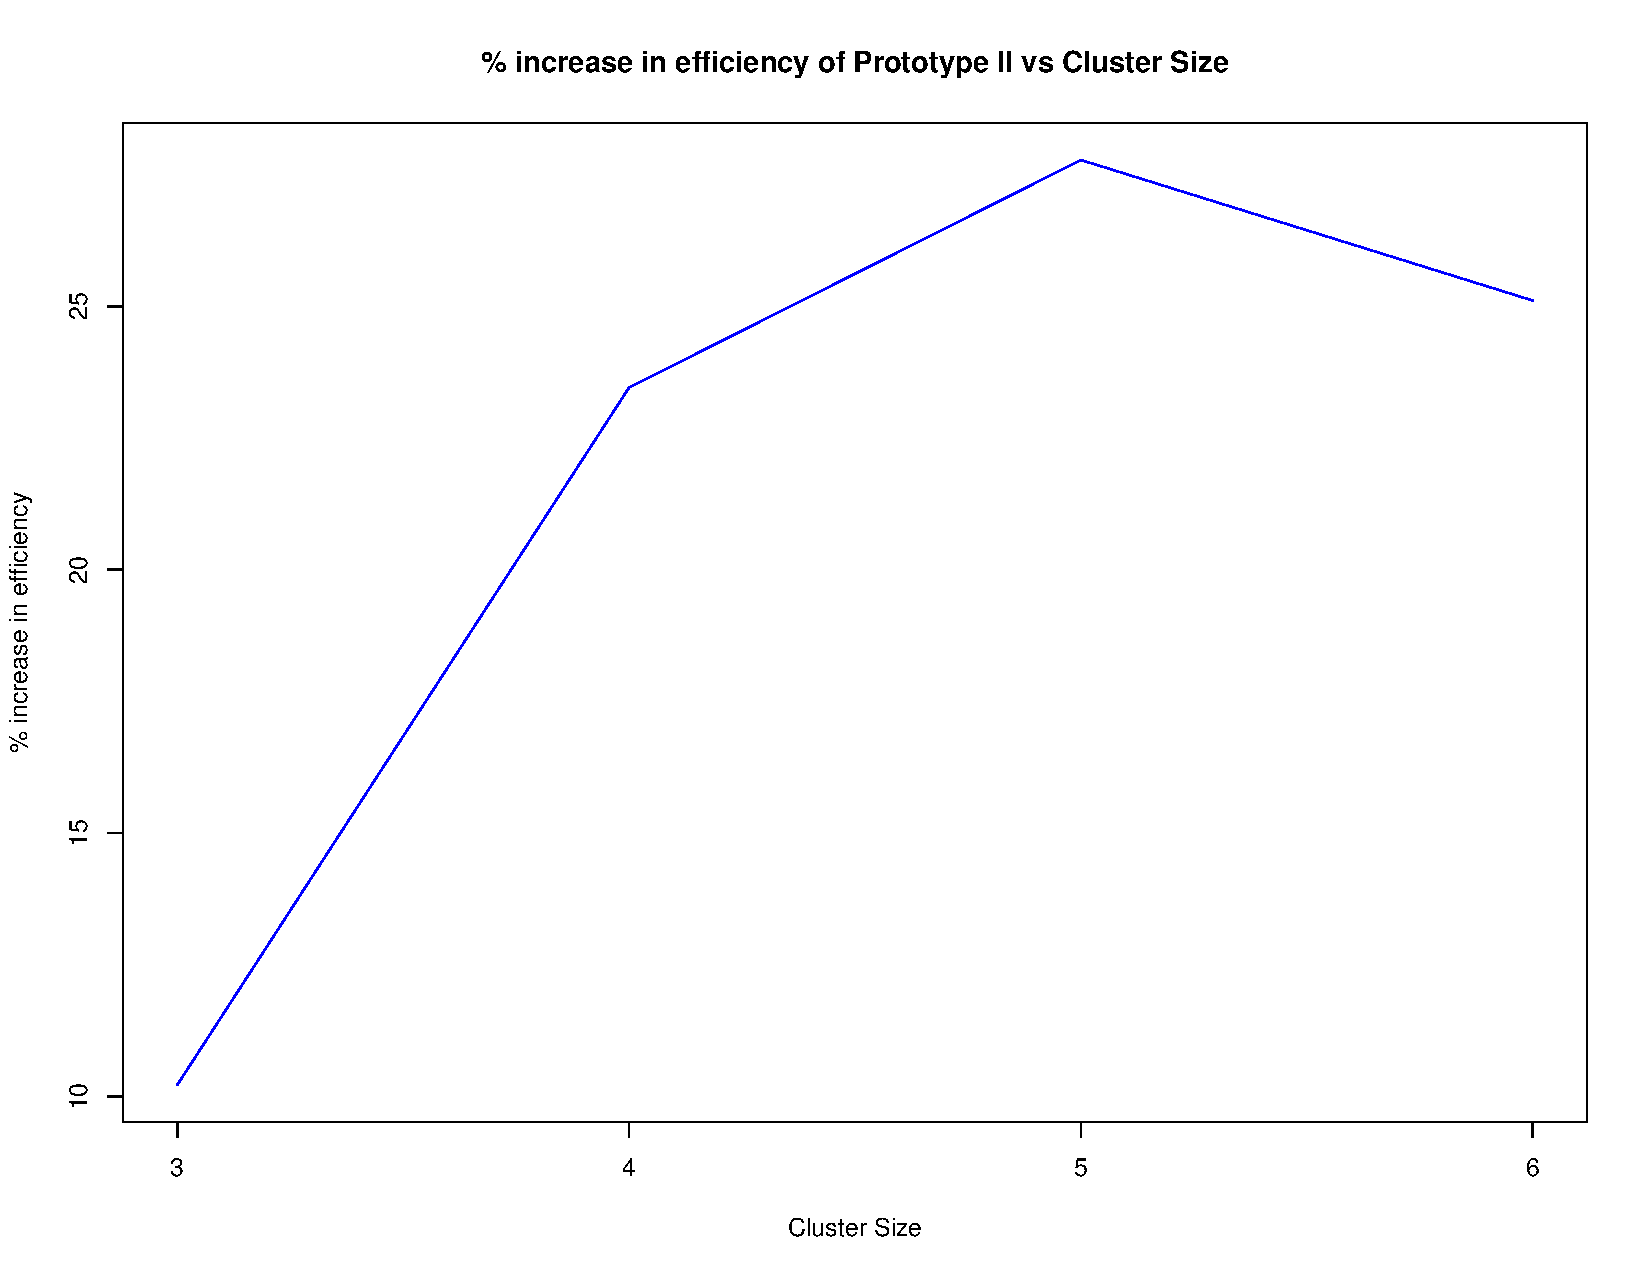
\includegraphics[scale=0.5]{perInceffProtoIIvsClusterSize.pdf}
\caption{ Percentage increase in Efficiency of Prototype II Vs Cluster Size For Same Models Input Set}
\label{fig:perInceffProtoIIvsCS}
\end{subfigure}
\end{figure}

\begin{figure}
\centering
\captionsetup[subfigure]{labelformat=empty}
\begin{subfigure}
\centering
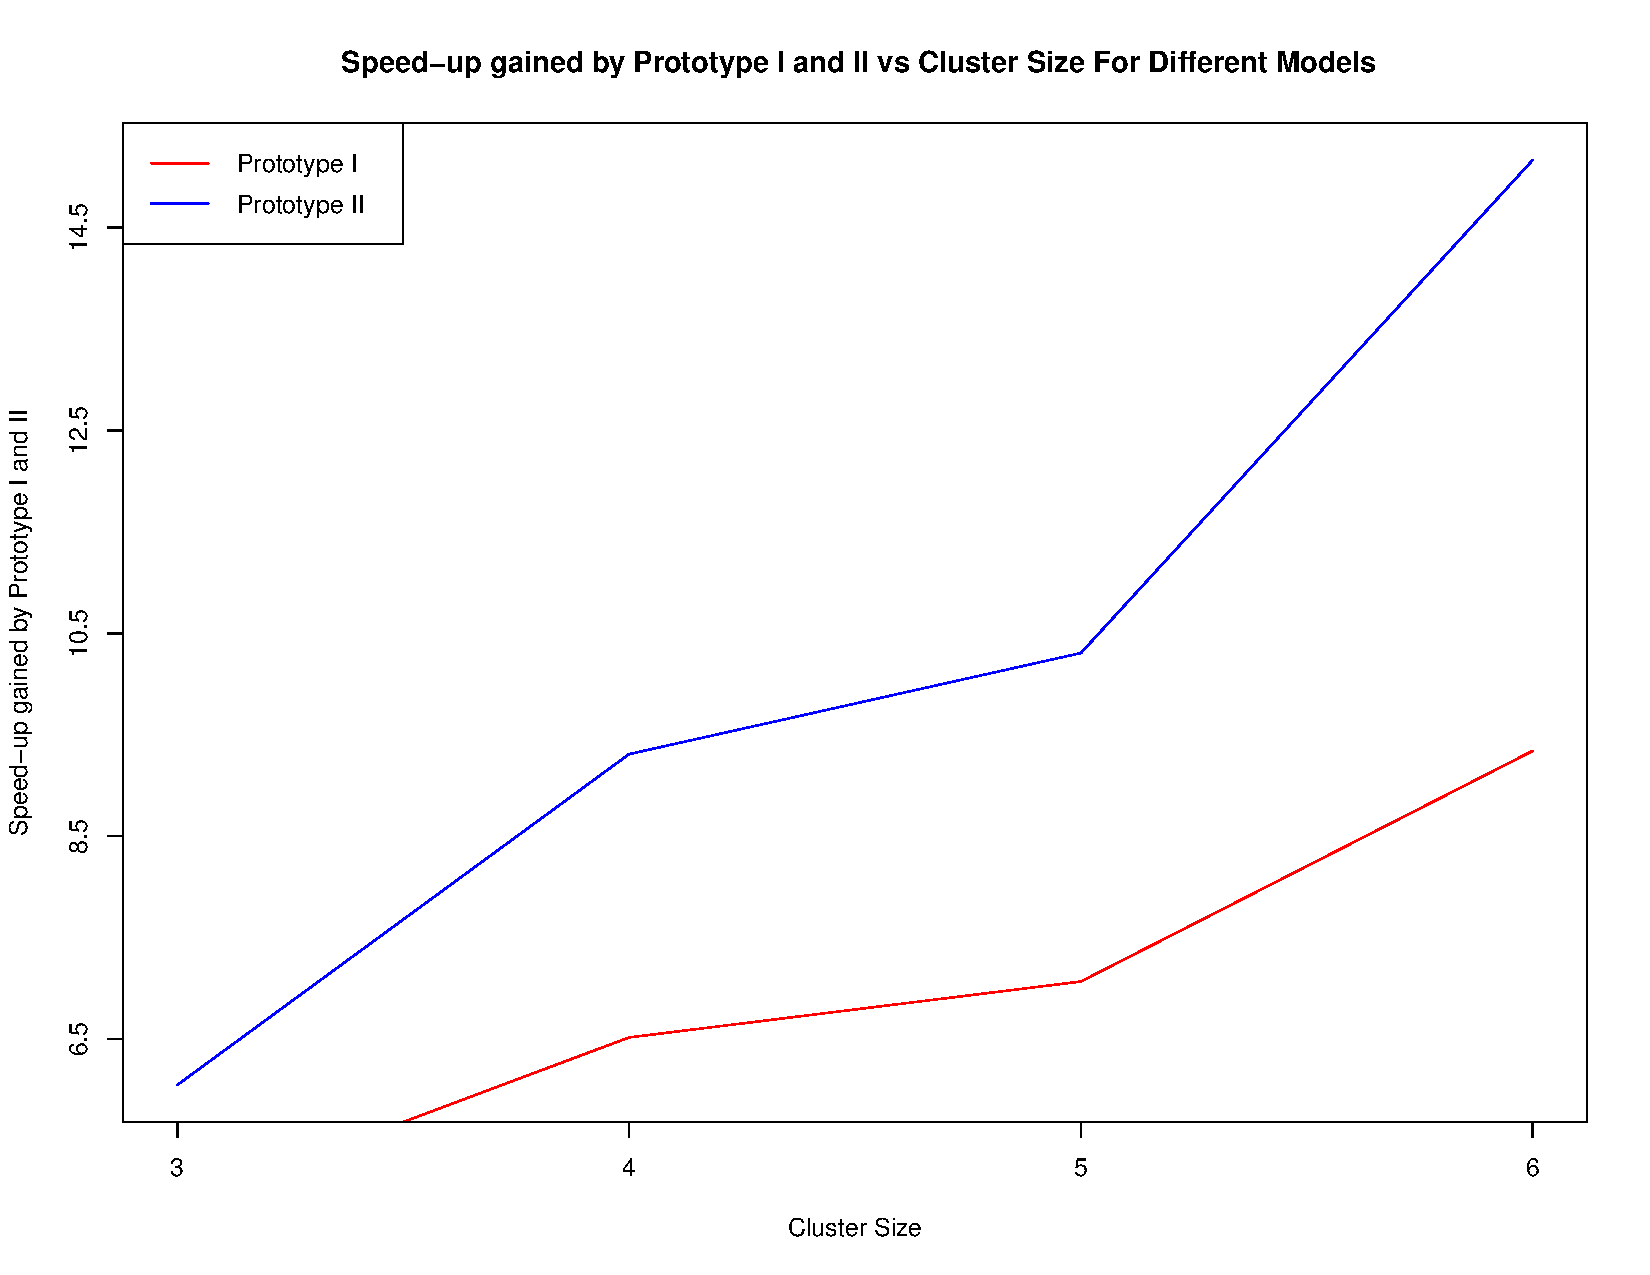
\includegraphics[scale=0.5]{SpeedUpProtoIProtoIIVsCS.pdf}
\caption{Speed-up of Prototype I and II Vs Cluster Size For Different Models Input Set}
\label{fig:SUPIPIvsCS}
\end{subfigure}
\begin{subfigure}
\centering
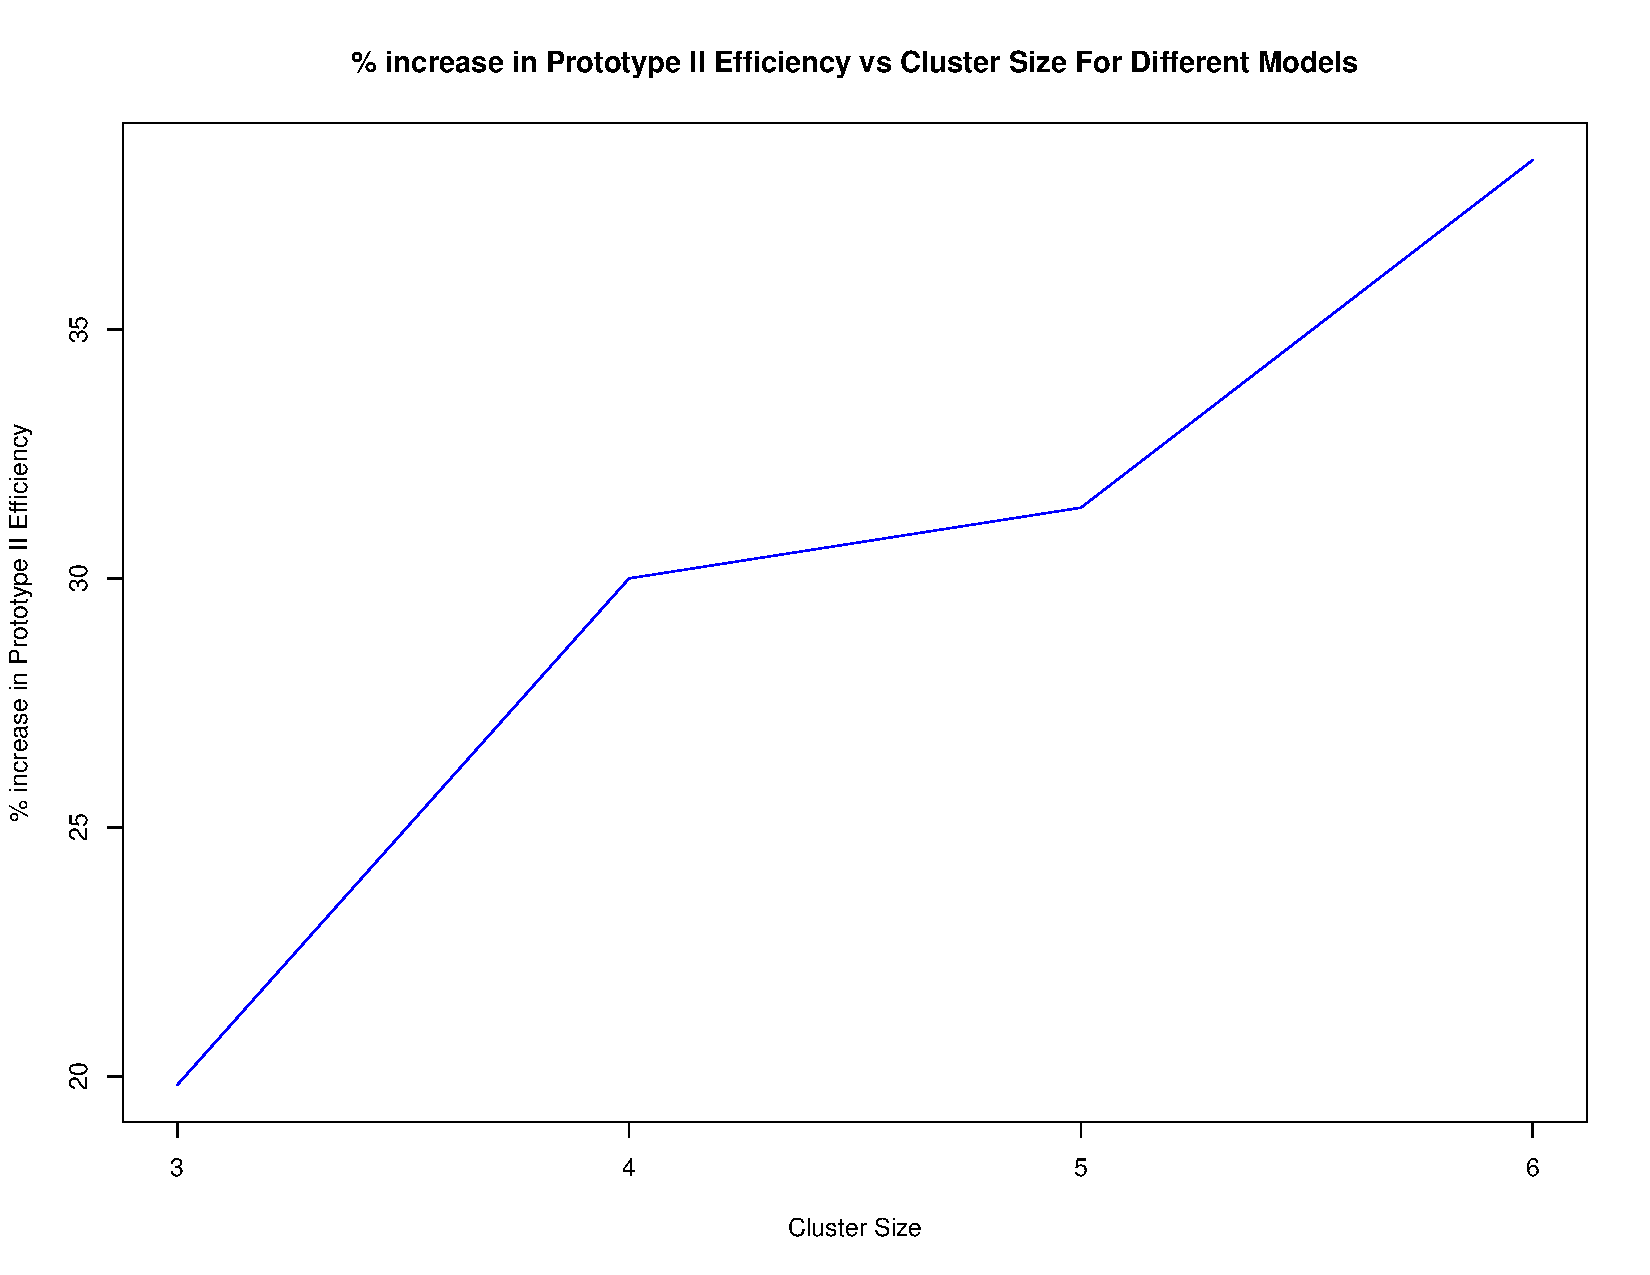
\includegraphics[scale=0.5]{PerIncEffofProtoIIVsCS.pdf}
\caption{ Percentage increase in Efficiency of Prototype II Vs Cluster Size For Different Models Input Set}
\label{fig:PerIncEffofProtoIIVsCS}
\end{subfigure}
\end{figure}

\begin{figure}
\centering
\captionsetup[subfigure]{labelformat=empty}
\begin{subfigure}
\centering
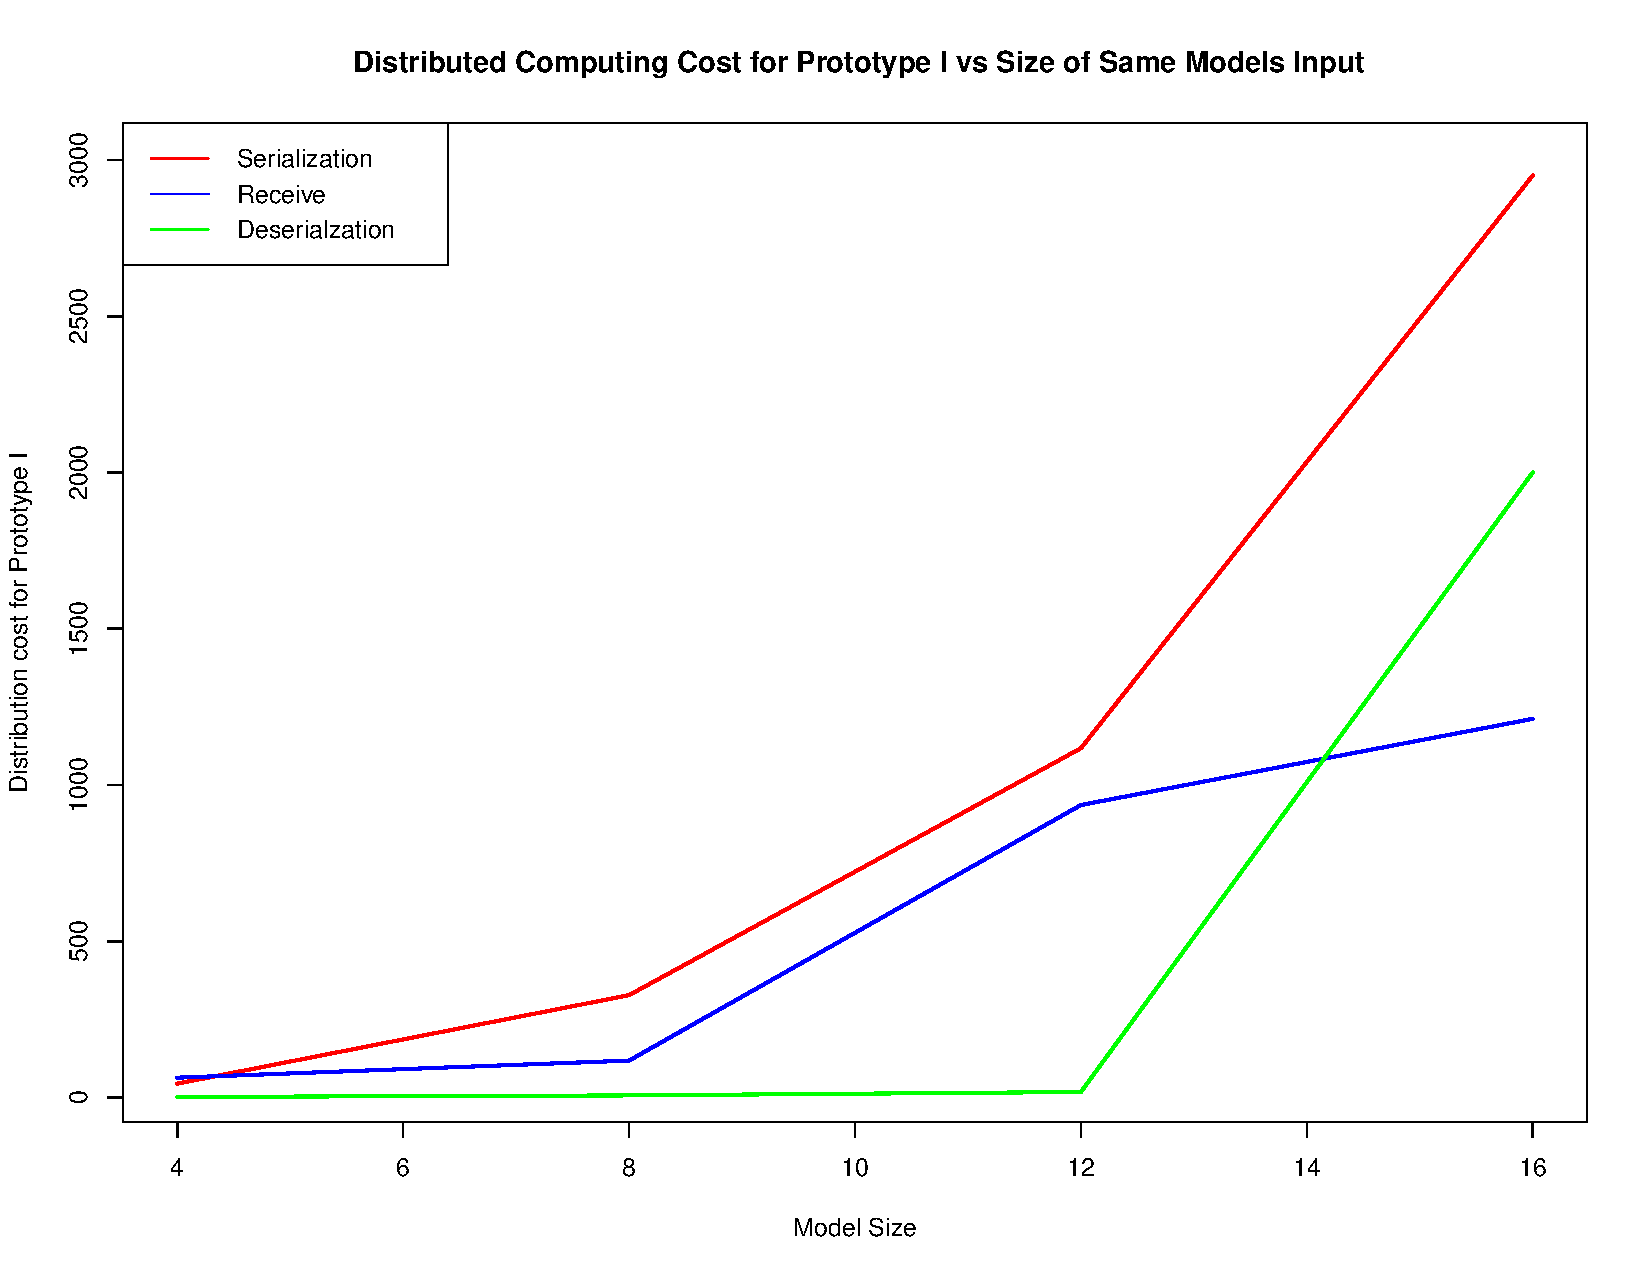
\includegraphics[scale=0.5]{DCPIvsCS.pdf}
\caption{Distributed Computing Cost for Prototype I vs Model Size}
\label{fig:PIDCCS}
\end{subfigure}
\begin{subfigure}
\centering
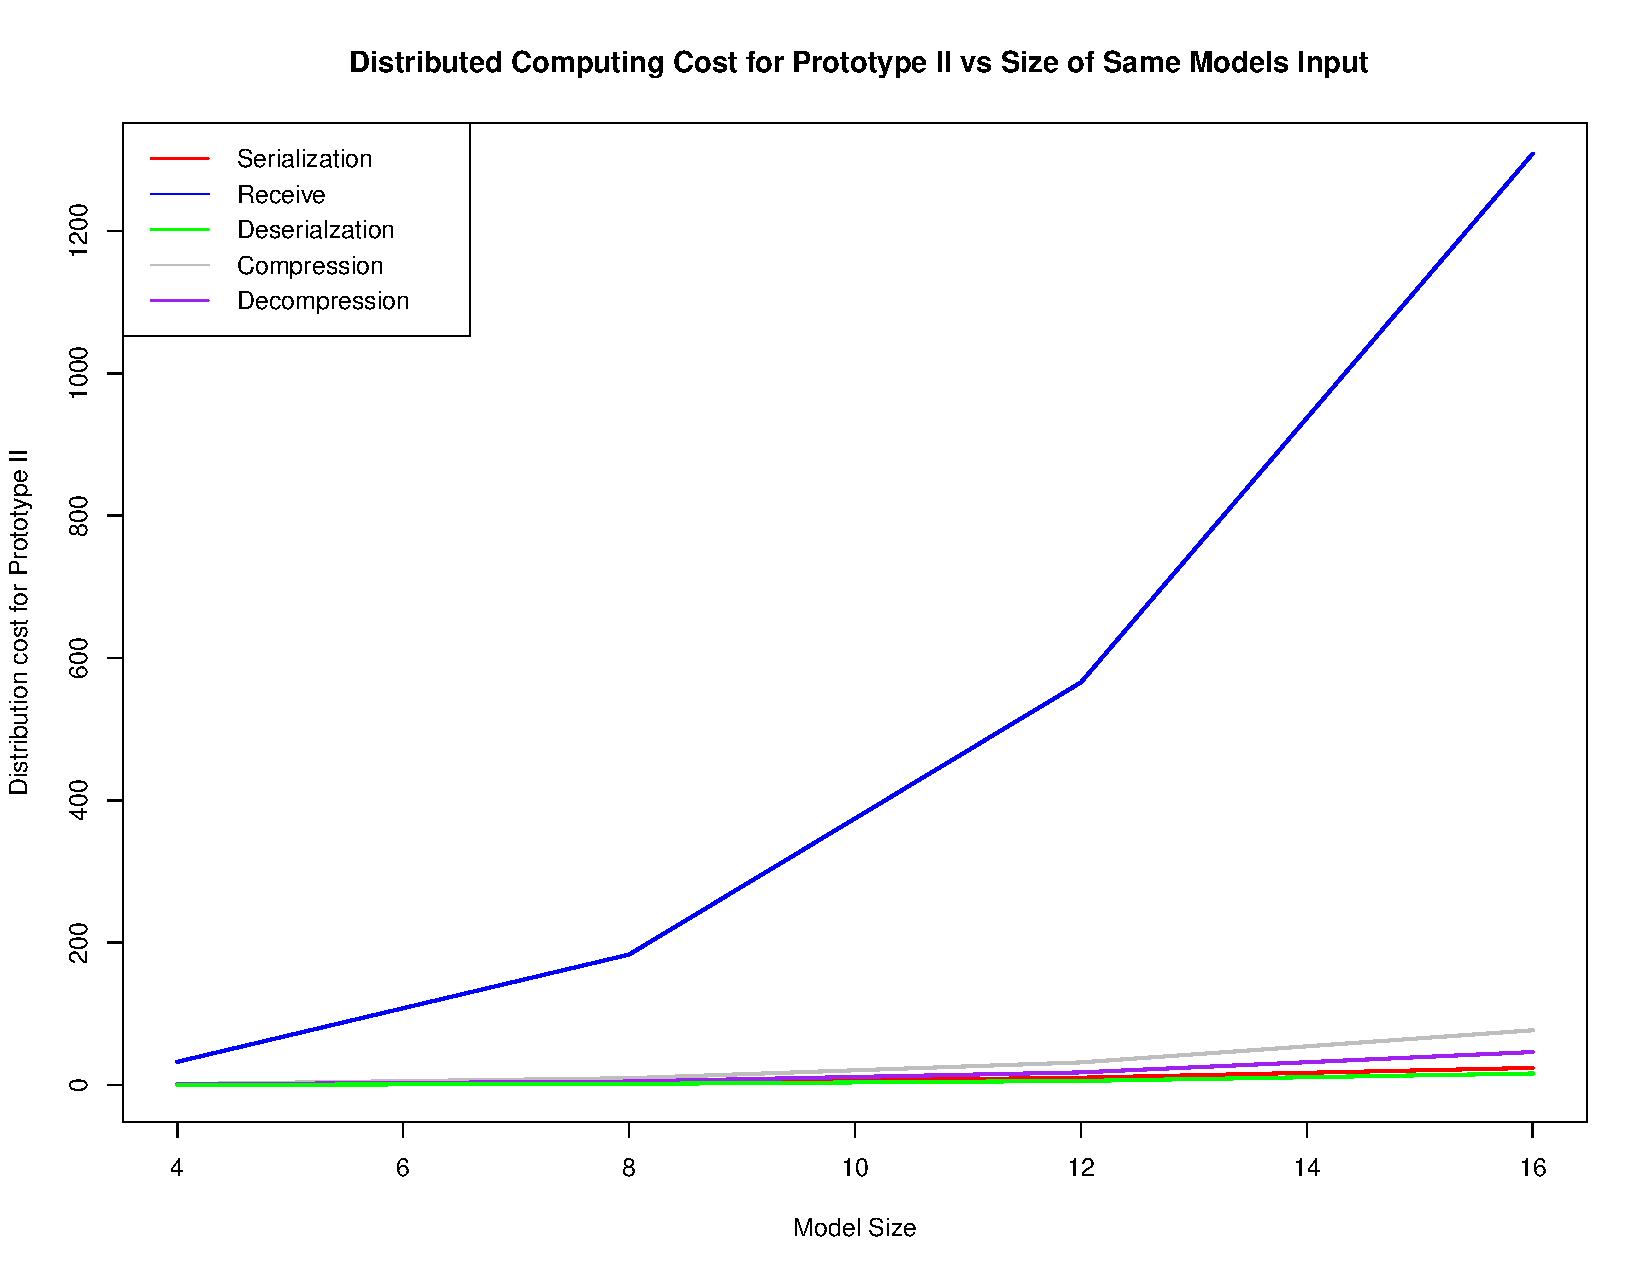
\includegraphics[scale=0.5]{DCPIIvsSize.pdf}
\caption{ Distributed Computing Cost for Prototype II vs Model Size}
\label{fig:PIIDCSize}
\end{subfigure}
\end{figure}

\begin{enumerate}
\item \textbf{Test-Scenario}: To understand how well the prototypes perform with increase in the cluster size, the distributed cuttlefish prototype I and prototype II were executed with constant load by adding a slave node for each test. There were 5 runs per test with the distributed system having 3, 4, 5, 6 cluster size respectively.
\begin{itemize}
\item \textbf{Tests-Data}: The whole test-case was executed with two input sets, one input set consisted of 10 head models and the second set consisted of the 5 head and 5 dame models. Each model was 8cm and resolution used was \begin{math}300 \times 150 \times 470 \end{math}.  
\item \textbf{Results}: The Table \ref{ProtoIVsProtoII-CS} and Table \ref{ProtoIVsProtoII-CSDiffModels}  summarizes the total execution time for both the prototypes for varying cluster size, speed-up gained by the prototypes in comparison to the non-distributed cuttlefish execution and efficiency of the prototypes for varying cluster size for same and different models input set. The Figure \ref{fig:SUPIPII} depicts the speed-up gained by each of the prototypes with increase in cluster size for a given workload for same model input and Figure \ref{fig:perInceffProtoIIvsCS}  shows that increase in the efficiency of the prototype II in comparison to efficiency of prototype I. The Figure \ref{fig:SUPIPIvsCS} depicts the speed-up gained by each the prototypes with increase in cluster size for a given workload for different models input and and Figure \ref{fig:PerIncEffofProtoIIVsCS} shows the increase in the efficiency of the prototype II in comparison to efficiency of prototype I .
\item \textbf{Observation}: The difference between the speed-up gained by Prototype II and I increases with the increase in the cluster size, showing that Prototype II scales well with increase in cluster size for given workload in comparison to the Prototype I. The percentage increase in efficiency in the Prototype II increases with cluster size even though not at a constant rate. 
\end{itemize}

\item \textbf{Test-Scenario}: To understand how well the prototypes perform with increase in the size of the models, the distributed cuttlefish prototype I and prototype II were executed with constant number but varying size of models and cluster size . 
\begin{itemize}
\item \textbf{Tests-Data}: There were 5 runs per test with 5 head models with size 4cm, 8cm, 12cm, and 16cm executed in a distributed systems of 5 nodes and \begin{math} 300 \times 150 \times 470 \end{math} resolution.  
\item \textbf{Results}: The Table \ref{DCPIvsModSize} summarizes the total execution time, time taken to perform serialization by the slowest slave node, time taken by the master node slowest worker thread to perform deserialization and time taken to receive partial output for Prototype I. The Table \ref{DCPIIvsModSize} summarizes the total execution time, time taken to perform serialization and compression by the slowest slave node, time taken by the master node slowest worker thread to perform deserialization, decompression and time taken to receive partial output for Prototype II.
\item \textbf{Observation}: The Figure \ref{fig:RTvsSize} shows that the execution time for both the prototypes increases with increase in model size. The model size determines the number of slices and size of the slices, therefore increase in model size leads to more workload per slave node in the cluster. As previously discussed Prototype II performs better than Prototype I. The cost of distributed computing is the sum of time periods spent in performing actions specific to distributed computing i.e. communication amongst the cluster nodes, serialization and deserialization of slices, and compression and decompression of slices (specific to Prototype II). In Prototype I, Figure \ref{fig:PIDCCS}, the time spent in partial output communication is lesser than Prototype I, Figure \ref{fig:PIIDCSize}, where as the serialization cost is higher in Prototype I as the serialized data is written to the network file system i.e. disk I/O.    
\end{itemize}
\end{enumerate}


\begin{figure}[t]
\centering
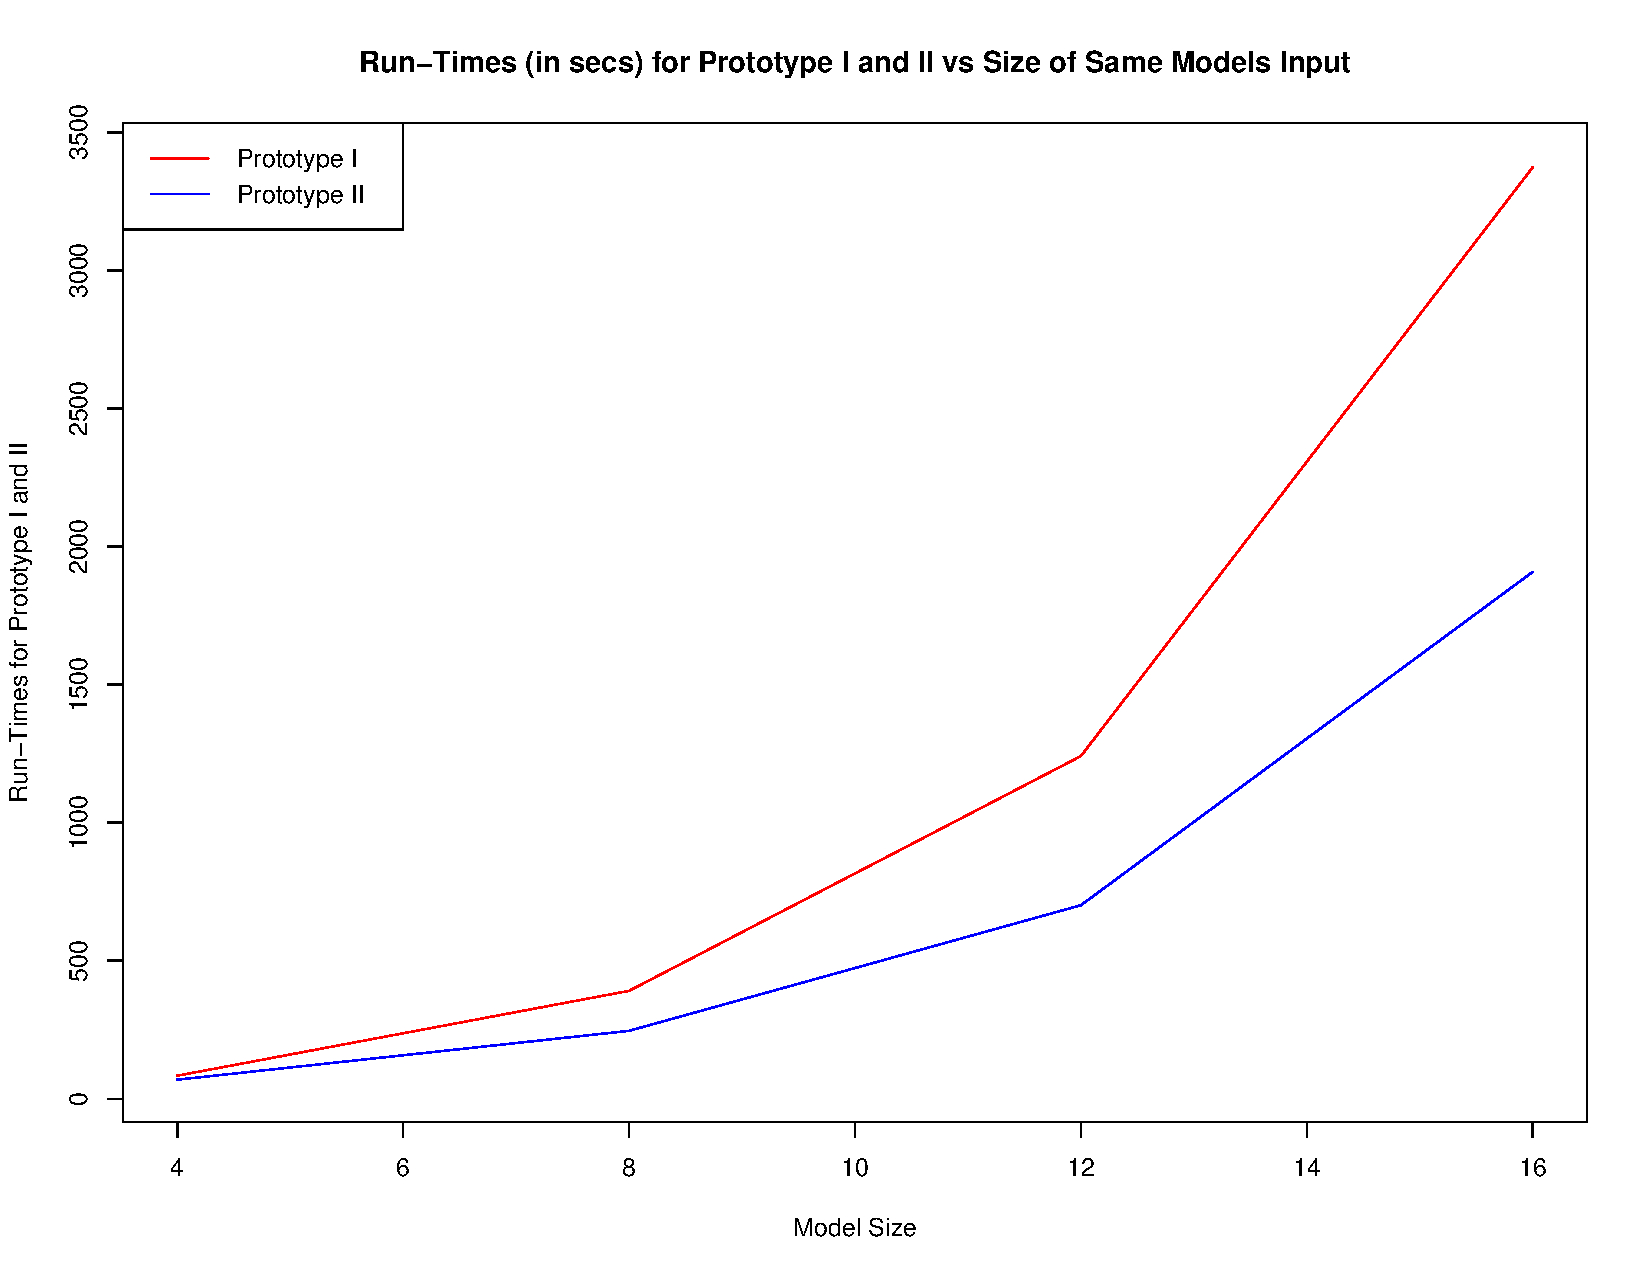
\includegraphics[scale=0.5]{PIP2RTvsSize.pdf}
\caption{Total Execution Time for Prototype I and II vs Model Size}
\label{fig:RTvsSize}
\end{figure}

\begin{table}
\centering
\caption{Prototype I vs Prototype II Measurements for 10 Head Models}
\label{ProtoIVsProtoII-CS}
\scalebox{0.9}{
\begin{tabular}{|l|l|l|l|l|l|l|l|}
\hline
\multicolumn{1}{|c|}{\textbf{\begin{tabular}[c]{@{}c@{}}Cluster\\ Size\end{tabular}}} & \multicolumn{1}{c|}{\textbf{\begin{tabular}[c]{@{}c@{}}Total \\ Execution \\ Time for\\ Prototype I\end{tabular}}} & \multicolumn{1}{c|}{\textbf{\begin{tabular}[c]{@{}c@{}}Total \\ Execution \\ Time \\ for\\ Prototype II\end{tabular}}} & \multicolumn{1}{c|}{\textbf{\begin{tabular}[c]{@{}c@{}}Total \\ Execution\\ Time by \\ Non-Distributed\\ Cuttlefish\end{tabular}}} & \multicolumn{1}{c|}{\textbf{\begin{tabular}[c]{@{}c@{}}Prototype\\       I\\ Speed-up\end{tabular}}} & \multicolumn{1}{c|}{\textbf{\begin{tabular}[c]{@{}c@{}}Prototype \\       II\\ Speed-up\end{tabular}}} & \multicolumn{1}{c|}{\textbf{\begin{tabular}[c]{@{}c@{}}Efficiency\\ of \\ Prototype I\end{tabular}}} & \multicolumn{1}{c|}{\textbf{\begin{tabular}[c]{@{}c@{}}Efficiency \\ of \\ Prototype II\end{tabular}}} \\ \hline
3                                                                                     & 1130.51                                                                                                           & 1014.98                                                                                                              & 4790.19                                                                                                                           & 4.23                                                                                                & 4.71                                                                                                 & 1.41                                                                                          & 1.57                                                                                            \\ \hline
4                                                                                     & 917.45                                                                                                            & 702.24                                                                                                               & 4790.19                                                                                                                           & 5.22                                                                                               & 6.82                                                                                                 & 1.30                                                                                          & 1.70                                                                                            \\ \hline
5                                                                                     & 675.97                                                                                                           & 488.21                                                                                                               & 4790.19                                                                                                                           & 7.08                                                                                               & 9.81                                                                                                 & 1.41                                                                                          & 1.96                                                                                            \\ \hline
6                                                                                     & 555.87                                                                                                           & 416.29                                                                                                               & 4790.19                                                                                                                           & 8.61                                                                                               & 11.50                                                                                                 & 1.43                                                                                          & 1.91                                                                                            \\ \hline
\end{tabular}}
\end{table}

\begin{table}
\centering
\caption{Prototype I vs Prototype II Measurements for Different Models Input}
\label{ProtoIVsProtoII-CSDiffModels}
\scalebox{0.9}{
\begin{tabular}{|l|l|l|l|l|l|l|l|}
\hline
\textbf{\begin{tabular}[c]{@{}l@{}}Cluster\\ Size\end{tabular}} & \multicolumn{1}{c|}{\textbf{\begin{tabular}[c]{@{}c@{}}Execution Time \\ for\\ Prototype I\end{tabular}}} & \multicolumn{1}{c|}{\textbf{\begin{tabular}[c]{@{}c@{}}Execution Time \\ for\\ Prototype II\end{tabular}}} & \multicolumn{1}{c|}{\textbf{\begin{tabular}[c]{@{}c@{}}Execution Time for\\ Non-Distributed \\ Cuttlefish\end{tabular}}} & \textbf{\begin{tabular}[c]{@{}l@{}}Speed-up\\ gained \\ by \\ Prototype I\end{tabular}} & \textbf{\begin{tabular}[c]{@{}l@{}}Speed-up\\ gained \\ by \\ Prototype II\end{tabular}} & \textbf{\begin{tabular}[c]{@{}l@{}}Efficiency\\ of \\ Prototype I\end{tabular}} & \textbf{\begin{tabular}[c]{@{}l@{}}Efficiency\\ of \\ Prototype II\end{tabular}} \\ \hline
3                                                               & 988.708                                                                                                   & 792.68                                                                                                   & 4793.47                                                                                                                  & 4.84                                                                                   & 6.04                                                                                    & 1.61                                                                           & 2.01                                                                            \\ \hline
4                                                               & 735.64                                                                                                  & 514.93                                                                                                    & 4793.47                                                                                                                  & 6.51                                                                                   & 9.30                                                                                    & 1.62                                                                           & 2.32                                                                            \\ \hline
5                                                               & 678.26                                                                                                  & 465.14                                                                                                   & 4793.47                                                                                                                  & 7.06                                                                                   & 10.30                                                                                   & 1.41                                                                           & 2.061                                                                            \\ \hline
6                                                               & 513.14                                                                                                  & 316.07                                                                                                    & 4793.47                                                                                                                  & 9.34                                                                                   & 15.16                                                                                   & 1.55                                                                          & 2.52                                                                            \\ \hline
\end{tabular}}
\end{table}

\begin{table}
\centering
\caption{Prototype I Performance For Varying Model Size}
\label{DCPIvsModSize}
\begin{tabular}{|l|l|l|l|l|}
\hline
\textbf{\begin{tabular}[c]{@{}l@{}}Model\\ Size\end{tabular}} & \textbf{\begin{tabular}[c]{@{}l@{}}Total Execution\\ time (in secs) for\\ Prototype I\end{tabular}} & \textbf{\begin{tabular}[c]{@{}l@{}}Time taken \\ for\\ Serialization\\  (in secs)\end{tabular}} & \textbf{\begin{tabular}[c]{@{}l@{}}Time taken\\ for\\ Receiving \\ Partial\\ Output (in secs)\end{tabular}} & \textbf{\begin{tabular}[c]{@{}l@{}}Time taken \\ for\\ Deserialization\\ (in secs)\end{tabular}} \\ \hline
4                                                             & 83.64                                                                                            & 44.25                                                                                         & 63.38                                                                                                    & 1.76                                                                                         \\ \hline
8                                                             & 390.95                                                                                           & 327.45                                                                                         & 118.12                                                                                                    & 6.68                                                                                          \\ \hline
12                                                            & 1241.23                                                                                       & 1117.58                                                                                        & 935.93                                                                                                     & 17.58                                                                                         \\ \hline
16                                                            & 3373.74                                                                                             & 2950.68                                                                                        & 1211.64                                                                                                   & 2000.62                                                                                        \\ \hline
\end{tabular}
\end{table}


\begin{table}
\centering
\caption{Prototype II Performance For Varying Model Size}
\label{DCPIIvsModSize}
\begin{tabular}{|l|l|l|l|l|l|l|}
\hline
\multicolumn{1}{|c|}{\textbf{\begin{tabular}[c]{@{}c@{}}Model\\ Size\end{tabular}}} & \multicolumn{1}{c|}{\textbf{\begin{tabular}[c]{@{}c@{}}Total Execution\\ time (in secs)\\ for\\ Prototype II\end{tabular}}} & \multicolumn{1}{c|}{\textbf{\begin{tabular}[c]{@{}c@{}}Time (in secs)\\  taken to \\ perform \\ serialization in\\  Prototype II\end{tabular}}} & \multicolumn{1}{c|}{\textbf{\begin{tabular}[c]{@{}c@{}}Time (in secs) \\ taken to\\ receive partial \\ output in \\ Prototype II\end{tabular}}} & \multicolumn{1}{c|}{\textbf{\begin{tabular}[c]{@{}c@{}}Time (in secs)\\  taken to\\ perform \\ deserialization \\ in Prototype II\end{tabular}}} & \multicolumn{1}{c|}{\textbf{\begin{tabular}[c]{@{}c@{}}Time (in secs)\\ taken to \\ perform \\ compression \\ in Prototype II\end{tabular}}} & \multicolumn{1}{c|}{\textbf{\begin{tabular}[c]{@{}c@{}}Time (in secs)\\ taken to \\ perform \\ decompression\\  in Prototype II\end{tabular}}} \\ \hline
4                                                                                   & 69.17                                                                                                                    & 0.22                                                                                                                                       & 32.56                                                                                                                                        & 0.10                                                                                                                                        & 1.24                                                                                                                                      & 0.76                                                                                                                                      \\ \hline
8                                                                                   & 246.19                                                                                                                    & 2.65                                                                                                                                        & 183.32                                                                                                                                        & 1.54                                                                                                                                         & 9.56                                                                                                                                     & 4.89                                                                                                                                       \\ \hline
12                                                                                  & 701.09                                                                                                                    & 10.23                                                                                                                                        & 565.80                                                                                                                                        & 5.70                                                                                                                                           & 31.76                                                                                                                                     & 17.72                                                                                                                                       \\ \hline
16                                                                                  & 1908.44                                                                                                                   & 24.04                                                                                                                                        & 1308.95                                                                                                                                        & 16.17                                                                                                                                         & 76.91                                                                                                                                     & 46.31                                                                                                                                       \\ \hline
\end{tabular}
\end{table}


\subsection{Distributed Cuttlefish Prototype II Performance Evaluation} \label{ProtoIIDesigns}

While implementing the distributed cuttlefish prototype II, two designs were possible for distribution of print jobs and merging of the partial slices. In each of the designs, the component configuration executed at the slave node is different. This difference in the component configuration of the pipeline executed on the salve node resulted in varying performance. As there was a significant difference in the performance, this Section is dedicated to explain how the decision of the component configuration impacts the overall performance of the application. It helped to gain insights about the impacts of the design on the performance which was discovered while performing the tests. \newline

In the first design, the transformation of the print objects in the print bed calculated by the \textit{PrintJobOrganizer} at the master is sent without modification to the slaves and the slaves generate the partial slices with print objects placed with the same transformation as sent by the master. This results in each slave generating partial slices with full slice height and width. At the master during merging process, the assigned material if not empty, is written from the partial slices to the full slices. After running the test-cases, it was seen that the performance of prototype II was comparatively bad with respect to prototype I. The major difference between the two prototypes is the communication of information between the master and slaves nodes. As the master nodes sent the print jobs having  print objects with the transformation, each of the slaves had to do processing of slices with the full slice height and width. Also, as each slave sent back the partial slices in form of stream of bytes, the size of the message to be sent increased considerably given that each partial slice had the full slice dimension with material EMPTY\_VOXEL assigned to rest of the slice where there was no object placed.  To fix this performance issue, a new design of prototype II was implemented where in the slave nodes rearranged the print objects again by running the \textit{PrintJobOrganizer} component after receiving the print objects from the master. Due to this, new transformation for the print objects was applied which resulted in the partial slices being much smaller as the print objects were placed close to the origin and hence the messages (containing the serialized compressed slices) communicated by the slave nodes were smaller. \newline

\begin{table}
\centering
\caption{Prototype II: Design I vs Design II Different Models Input Set}
\label{ProtoIIDesignIVsDesignIIDiffMod}
\scalebox{0.8}{
\begin{tabular}{|c|c|c|c|l|c|c|}
\hline
\textbf{\begin{tabular}[c]{@{}c@{}}\# \\ Models \\ Head \\ \& \\ Dame\\ 8 cm\end{tabular}} & \textbf{\begin{tabular}[c]{@{}c@{}}Total Execution Time \\  (in secs) for \\ Distributed \\ Cuttlefish Prototype II\\ Design II- print objects with \\ transformation done \\ by master node\\ (Cluster Size- 3)\end{tabular}} & \textbf{\begin{tabular}[c]{@{}c@{}}Total Execution Time,\\ (in secs) for \\ Distributed \\ Cuttlefish Prototype II \\ Design I- print objects with \\ transformation done by \\ slave node\\ (Cluster Size- 3)\end{tabular}} & \textbf{\begin{tabular}[c]{@{}c@{}}Speed-up\\ in comparison to \\ the non-distributed \\ cuttlefish- \\ Design II\end{tabular}} & \multicolumn{1}{c|}{\textbf{\begin{tabular}[c]{@{}c@{}}Speed-up\\ in comparison \\ to the \\ non-distributed\\ cuttlefish-\\  Design I\end{tabular}}} & \textbf{\begin{tabular}[c]{@{}c@{}}Efficiency\\ Prototype II\\ -\\ Design II\end{tabular}} & \textbf{\begin{tabular}[c]{@{}c@{}}Efficiency \\ Prototype II\\ -\\ Design I\end{tabular}} \\ \hline
2                                                                                          & 94.52                                                                                                                                                                                                                       & 94.52                                                                                                                                                                                                                      & 2.58                                                                                                                     & 2.58                                                                                                                                              & 0.86                                                                                & 0.86                                                                                   \\ \hline
4                                                                                          & 181.95                                                                                                                                                                                                                       & 270.92                                                                                                                                                                                                                      & 3.49                                                                                                                     & 2.34                                                                                                                                              & 1.16                                                                                & 0.78                                                                                   \\ \hline
6                                                                                          & 357.61                                                                                                                                                                                                                        & 470.92                                                                                                                                                                                                                      & 3.27                                                                                                                     & 2.48                                                                                                                                              & 1.09                                                                                & 0.82                                                                                   \\ \hline
8                                                                                          & 492.65                                                                                                                                                                                                                       & 778.43                                                                                                                                                                                                                       & 3.83                                                                                                                     & 2.42                                                                                                                                              & 1.27                                                                                & 0.80                                                                                   \\ \hline
10                                                                                         & 792.68                                                                                                                                                                                                                       & 1951.24                                                                                                                                                                                                                      & 6.04                                                                                                                     & 2.45                                                                                                                                              & 2.01                                                                                & 0.81                                                                                   \\ \hline
\end{tabular}}
\end{table}

\begin{table}
\centering
\caption{Prototype II: Design I vs Design II Same Models Input Set}
\label{ProtoIIDesignIVsDesignIISameMod}
\scalebox{0.8}{
\begin{tabular}{|c|c|c|c|l|c|c|}
\hline
\textbf{\begin{tabular}[c]{@{}c@{}}\# \\ Models \\ Head \\ 8 cm\end{tabular}} & \textbf{\begin{tabular}[c]{@{}c@{}}Total Execution Time \\  (in secs) for \\ Distributed \\ Cuttlefish Prototype II\\ Design II- print objects with \\ transformation done \\ by master node\\ (Cluster Size- 3)\end{tabular}} & \textbf{\begin{tabular}[c]{@{}c@{}}Total Execution Time,\\ (in secs) for \\ Distributed \\ Cuttlefish Prototype II \\ Design I- print objects with \\ transformation done by \\ slave node\\ (Cluster Size- 3)\end{tabular}} & \textbf{\begin{tabular}[c]{@{}c@{}}Speed-up\\ in comparison to \\ the non-distributed \\ cuttlefish- \\ Design II\end{tabular}} & \multicolumn{1}{c|}{\textbf{\begin{tabular}[c]{@{}c@{}}Speed-up\\ in comparison \\ to the \\ non-distributed\\ cuttlefish-\\  Design I\end{tabular}}} & \textbf{\begin{tabular}[c]{@{}c@{}}Efficiency\\ Prototype II\\ -\\ Design II\end{tabular}} & \textbf{\begin{tabular}[c]{@{}c@{}}Efficiency \\ Prototype II\\ -\\ Design I\end{tabular}} \\ \hline
2                                                                             & 102.55                                                                                                                                                                                                                       & 135.49                                                                                                                                                                                                                       & 3.48                                                                                                                        & 2.63                                                                                                                                              & 1.16                                                                                   & 0.87                                                                                   \\ \hline
4                                                                             & 245.08                                                                                                                                                                                                                       & 345.342                                                                                                                                                                                                                      & 3.75                                                                                                                        & 2.66                                                                                                                                              & 1.25                                                                                   & 0.88                                                                                   \\ \hline
6                                                                             & 440.41                                                                                                                                                                                                                        & 594.30                                                                                                                                                                                                                     & 3.74                                                                                                                         & 2.77                                                                                                                                              & 1.24                                                                                    & 0.92                                                                                   \\ \hline
8                                                                             & 708.70                                                                                                                                                                                                                        & 1534.65                                                                                                                                                                                                                     & 5.74                                                                                                                        & 2.65                                                                                                                                               & 1.91                                                                                   & 0.88                                                                                    \\ \hline
10                                                                            & 1014.98                                                                                                                                                                                                                       & 1832.35                                                                                                                                                                                                                     & 4.71                                                                                                                        & 2.61                                                                                                                                              & 1.57                                                                                   & 0.87                                                                                    \\ \hline
\end{tabular}}
\end{table}

\begin{figure}
\centering
\captionsetup[subfigure]{labelformat=empty}
\begin{subfigure}
\centering
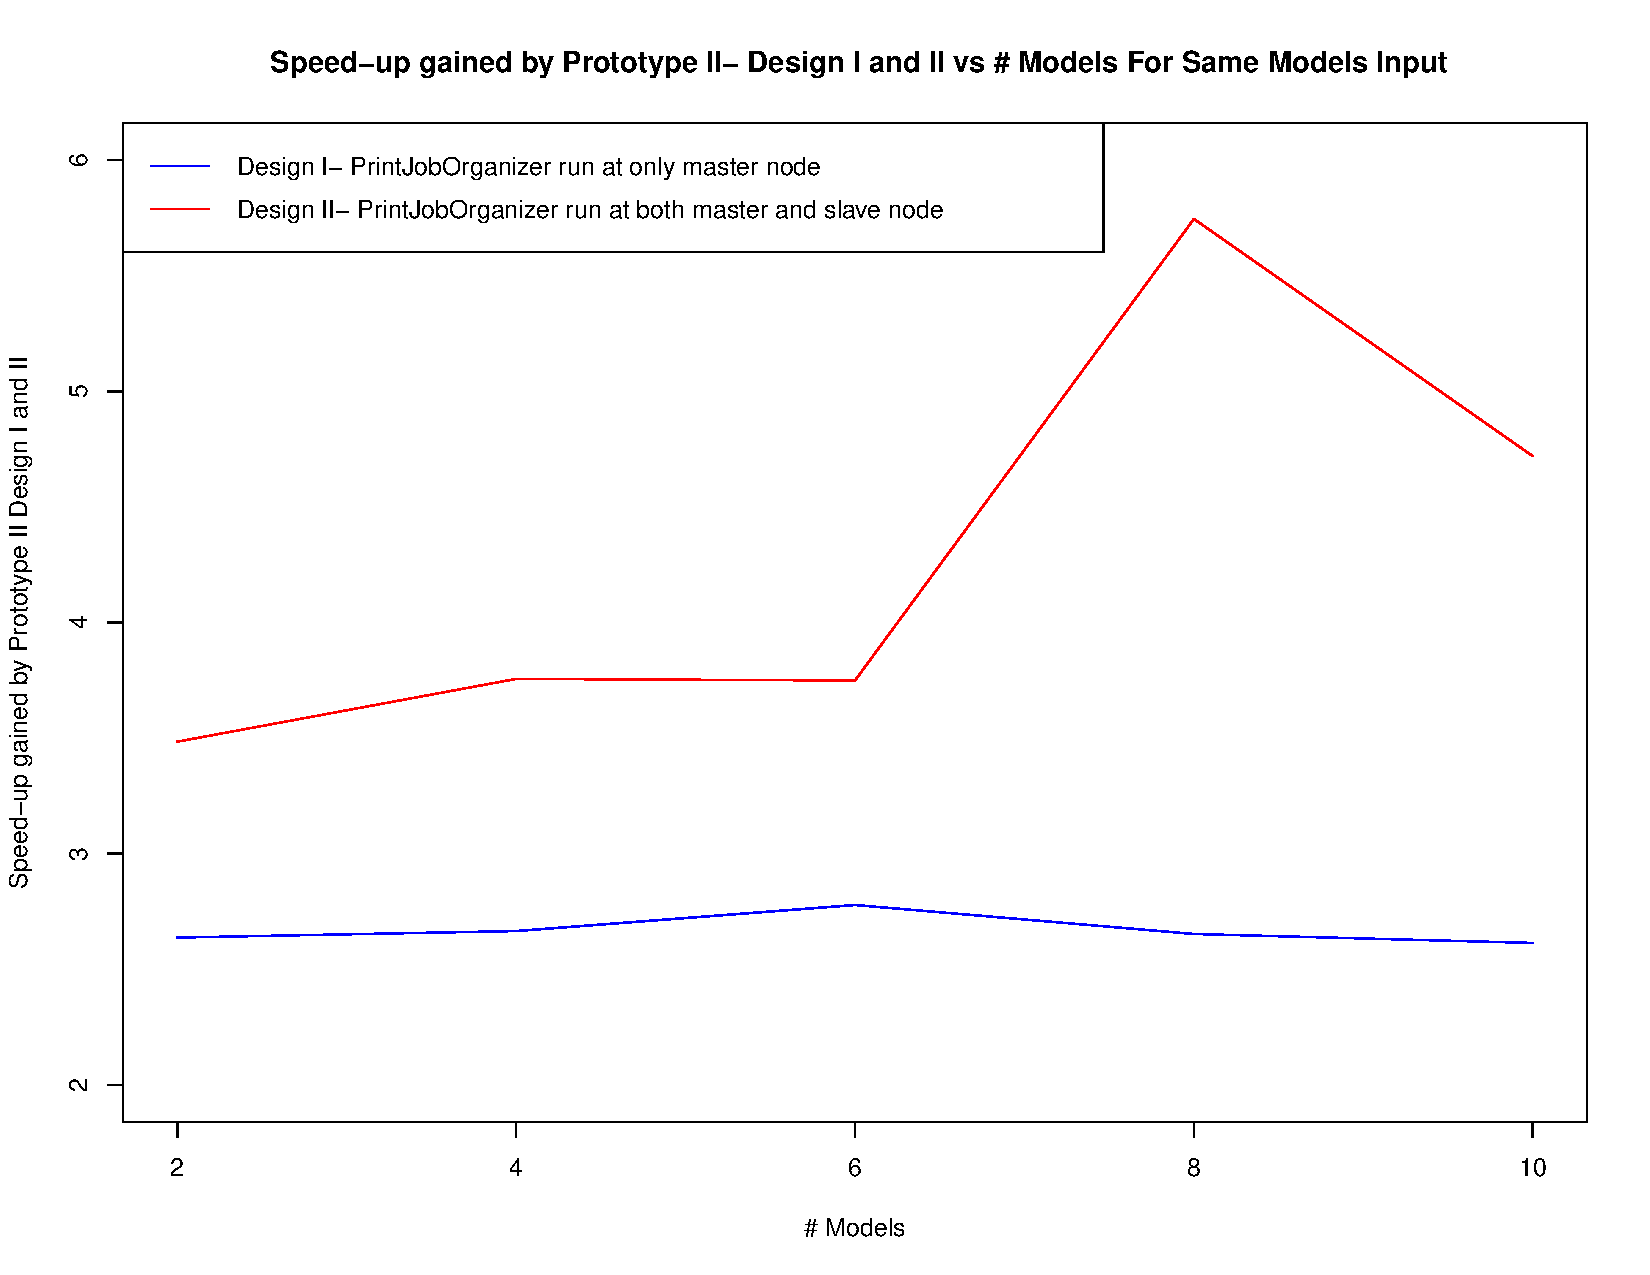
\includegraphics[scale=0.5]{SUDIDIIvsNumMod.pdf}
\caption{Speed-up of Design I and II Vs Number of Models For Same Models Input}
\label{fig:SUDIDIIvsNumMod}
\end{subfigure}
\begin{subfigure}
\centering
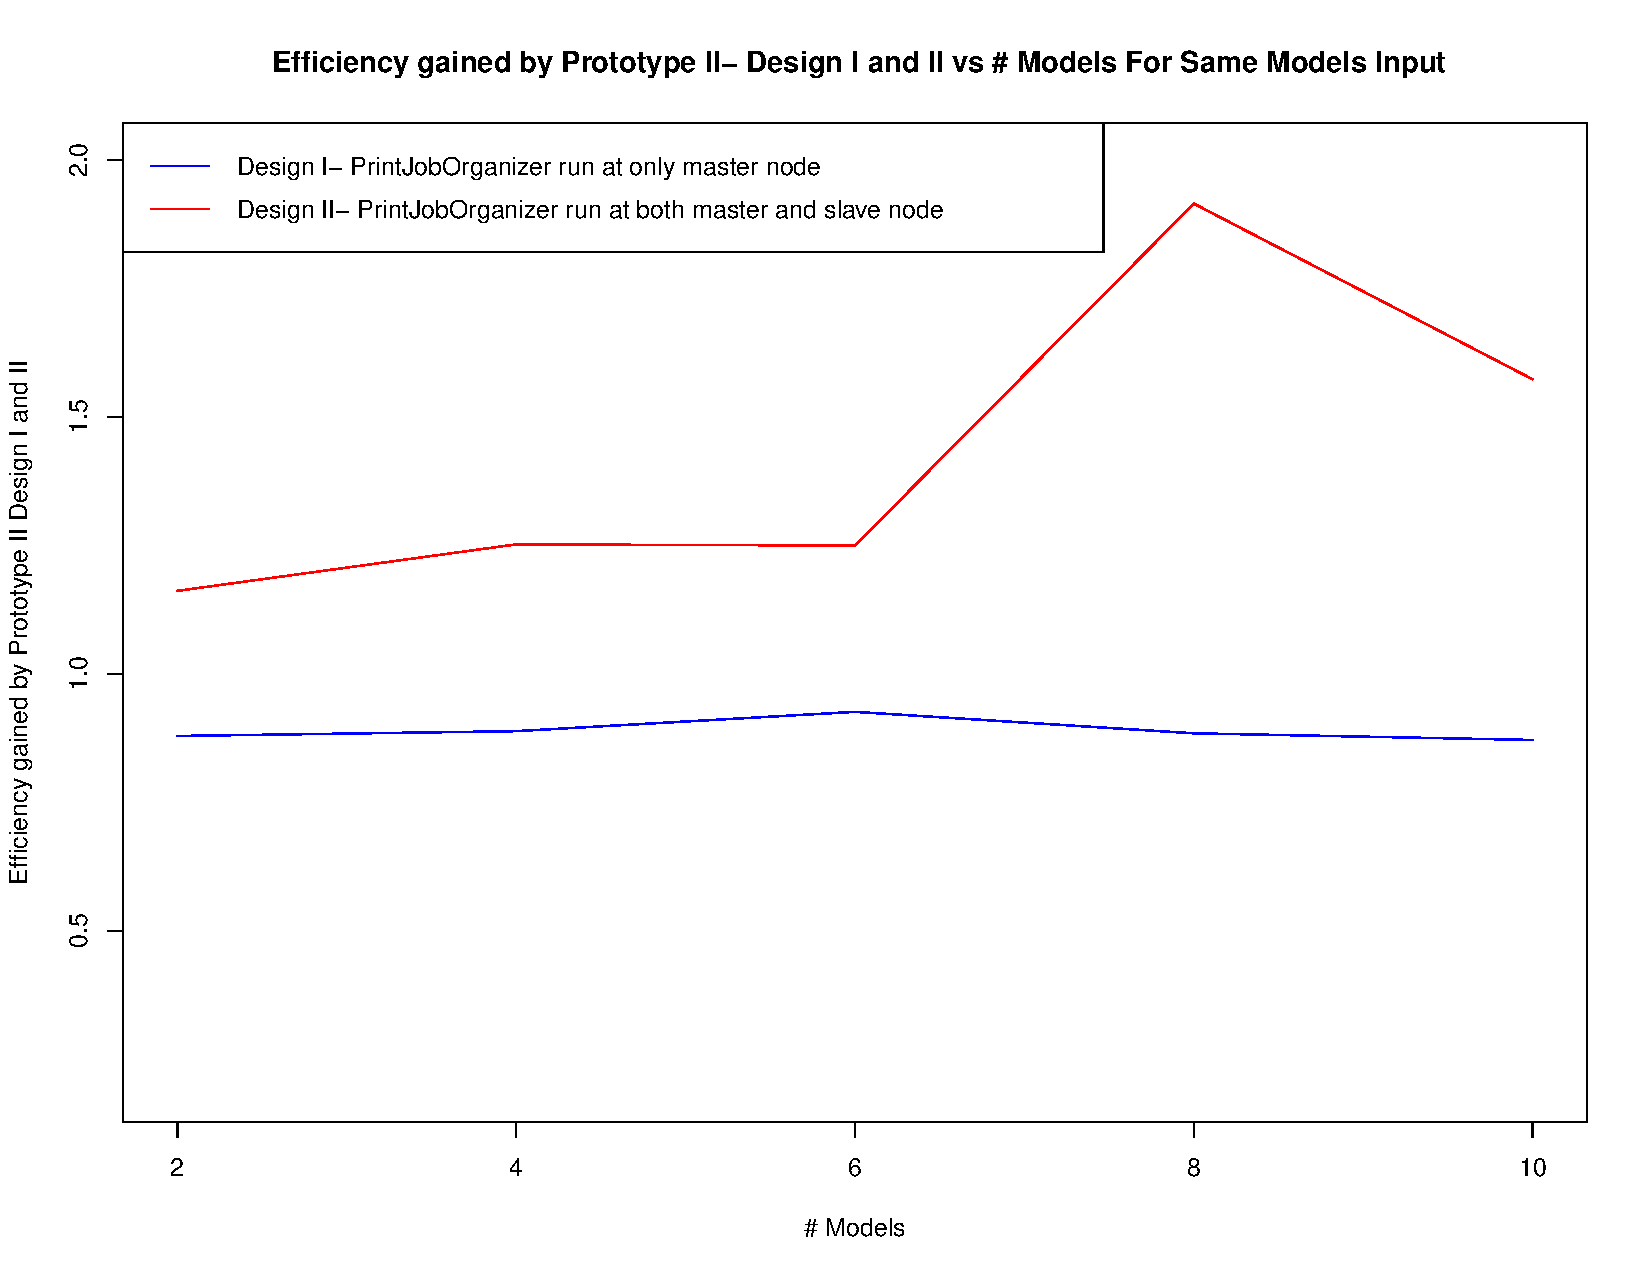
\includegraphics[scale=0.5]{EffDIDIIvsNumMod.pdf}
\caption{Efficiency of Design I and II Vs Number of Models For Same Models Input}
\label{fig:EffDIDIIvsNumMod}
\end{subfigure}
\end{figure}

\begin{figure}
\centering
\captionsetup[subfigure]{labelformat=empty}
\begin{subfigure}
\centering
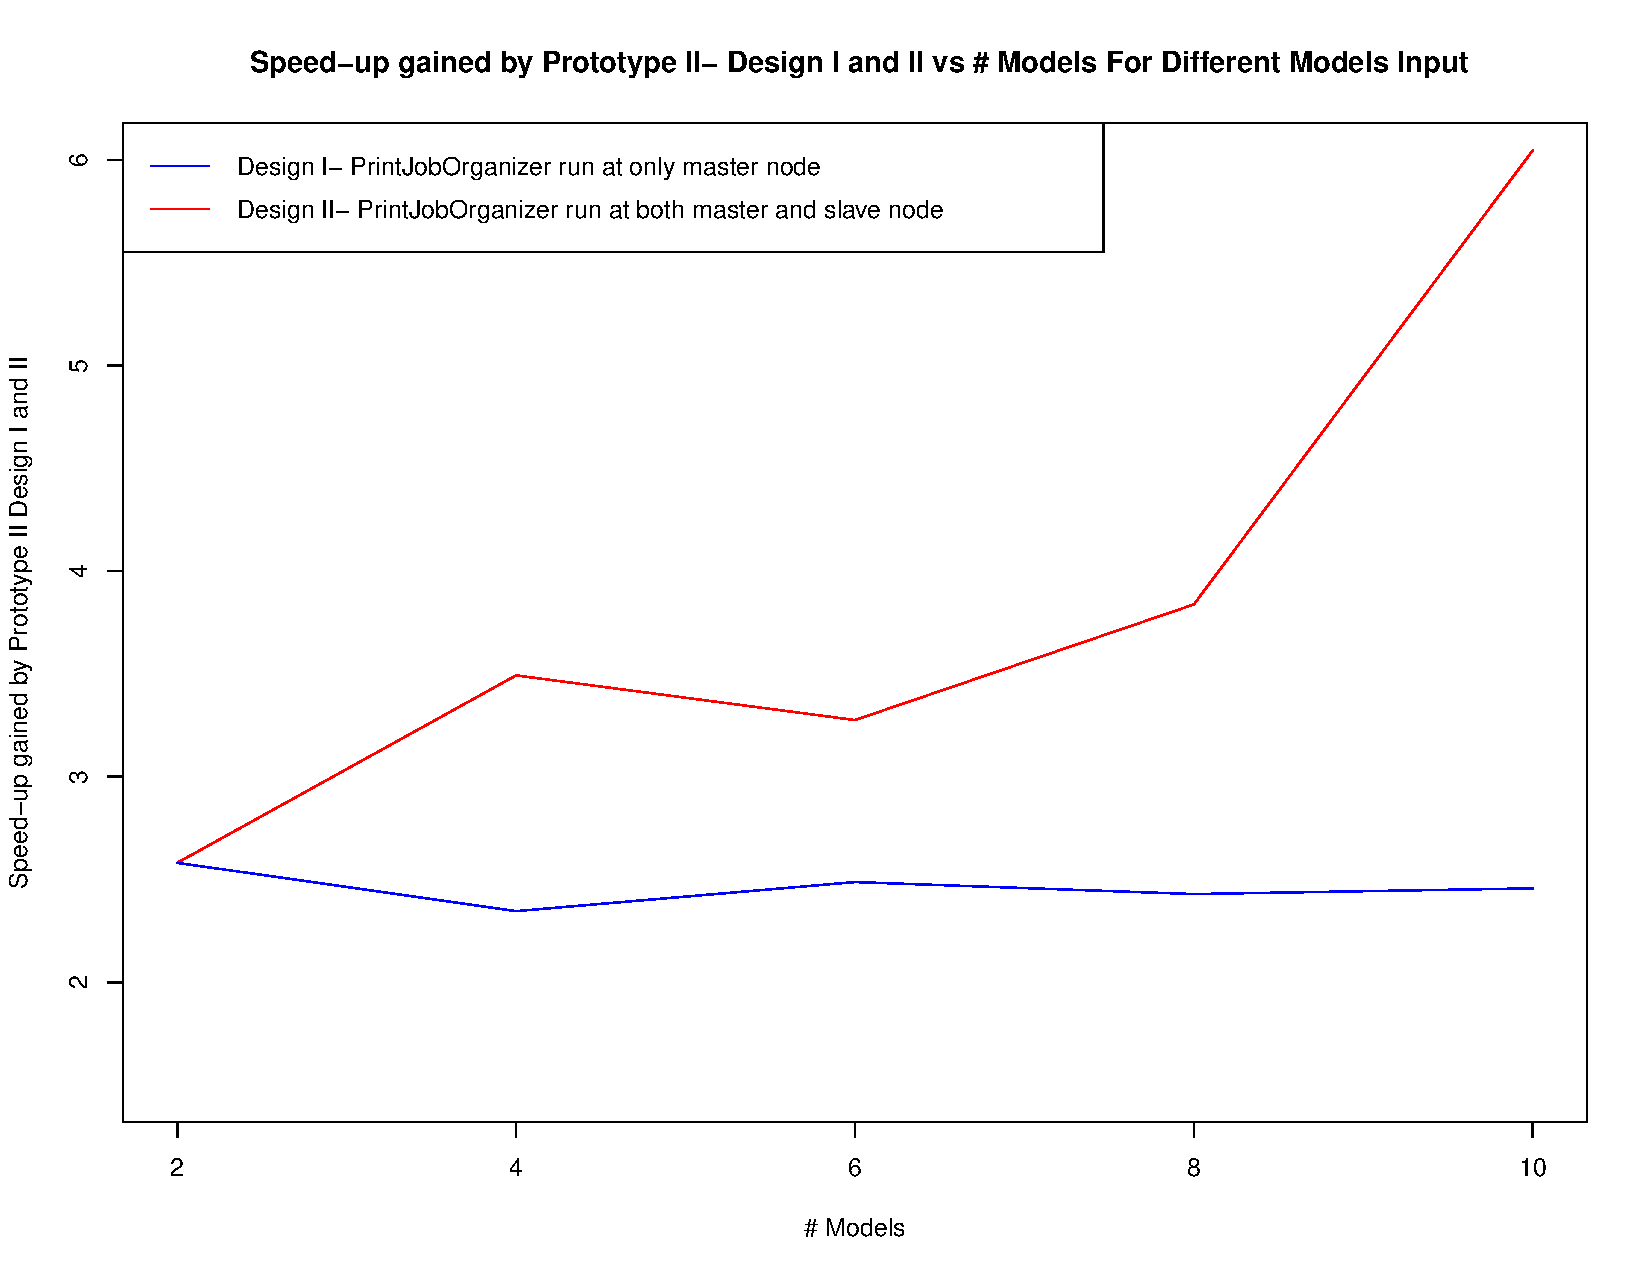
\includegraphics[scale=0.5]{SUDIDIIvsNumModDM.pdf}
\caption{Speed-up of Design I and II Vs Number of Models For Different Models Input}
\label{fig:SUDIDIIvsNumModDM}
\end{subfigure}
\begin{subfigure}
\centering
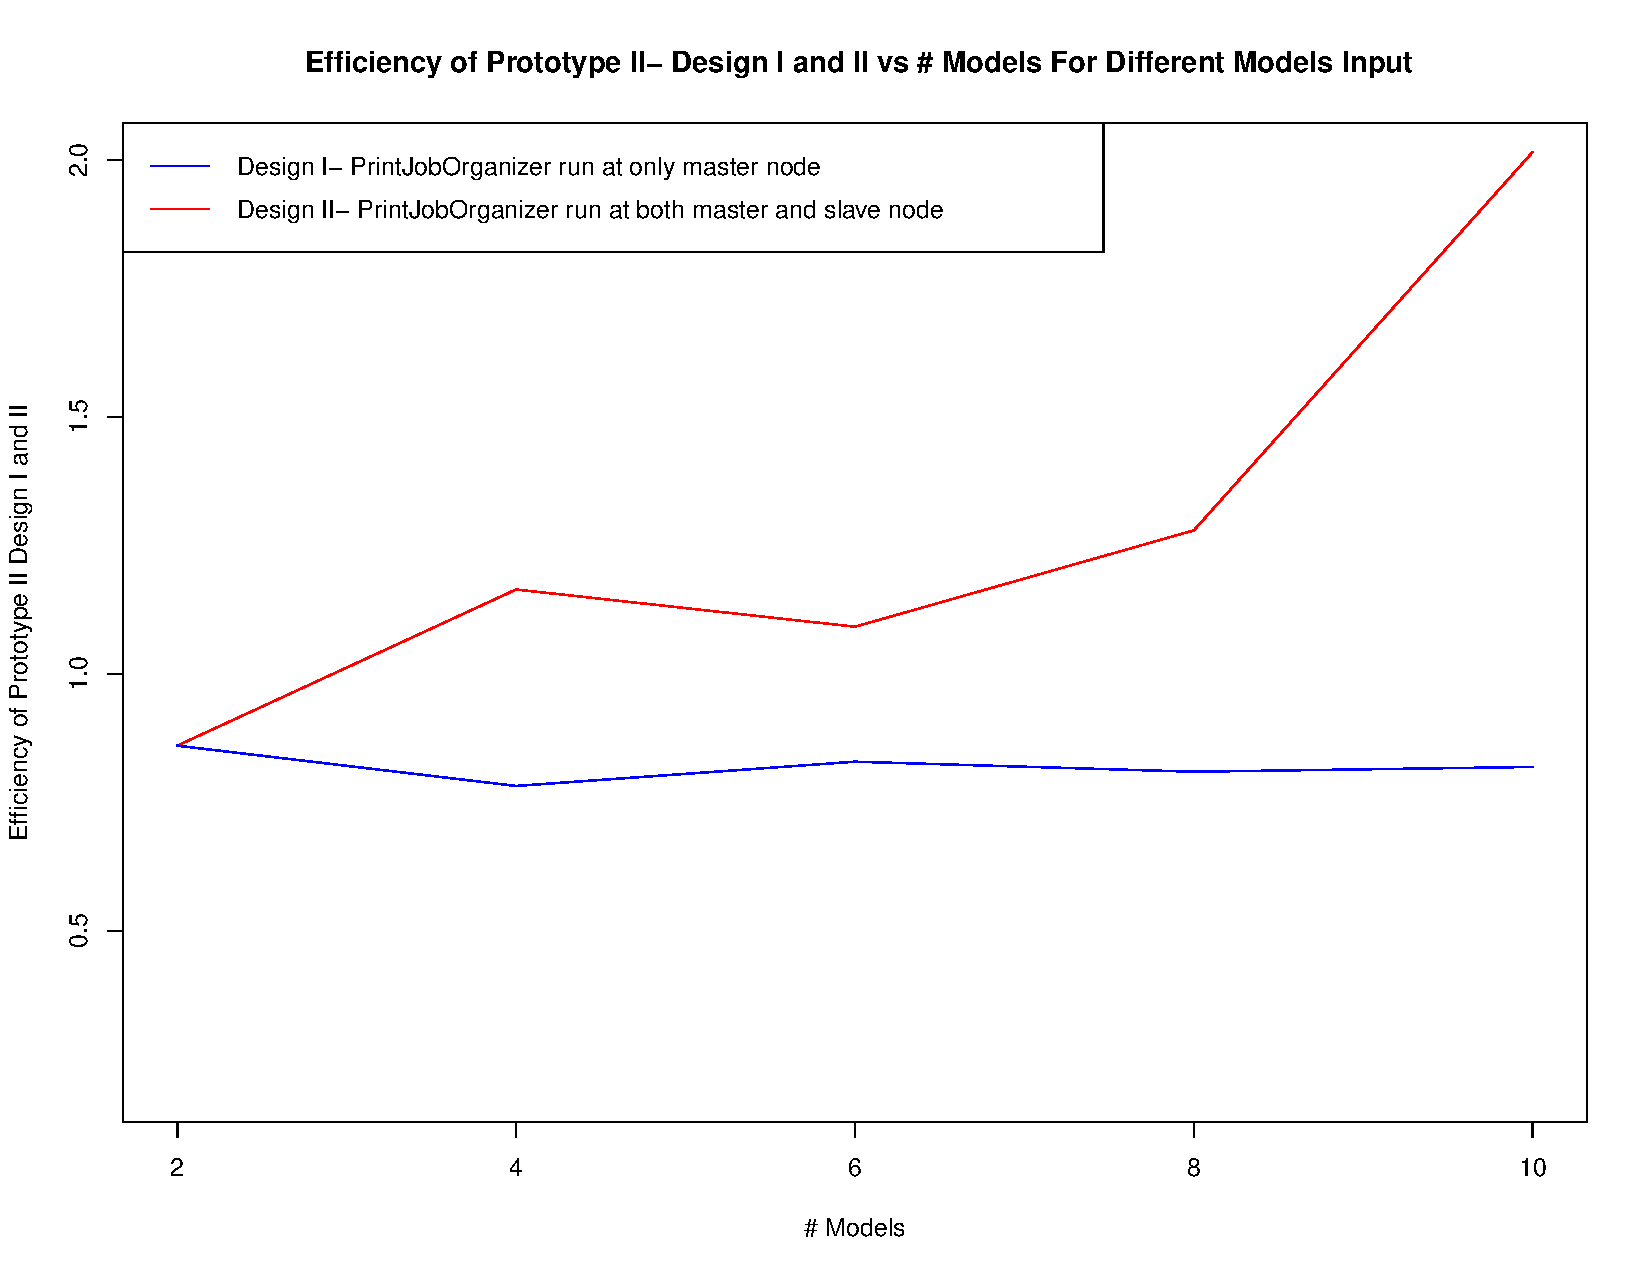
\includegraphics[scale=0.5]{EffDIDIIvsNumModDM.pdf}
\caption{Efficiency of Design I and II Vs Number of Models For Different Models Input}
\label{fig:EffDIDIIvsNumModDM}
\end{subfigure}
\end{figure}

\textbf{Test-Scenario}: To check the performance of two designs: The prototype II design I and design II were executed with a cluster of 3 nodes. The comparison of the two designs was done by comparing the speed-up achieved when compared with the non-distributed cuttlefish and the efficiency of the prototype II design II with varying workload. 
\begin{itemize}
\item \textbf{Test-Data}- The input set for the test-cases consisted of head models, 8cm each in the first set and second set consisted of head and dame model 8cm each. The resolution used was \begin{math} 300 \times 150 \times 470 \end{math}. 
\item \textbf{Results}- The Table \ref{ProtoIIDesignIVsDesignIIDiffMod} summarizes the execution times, speed-up and efficiency calculated for the two designs of prototype II for input set consisting of different models. The Table \ref{ProtoIIDesignIVsDesignIISameMod} summarizes the execution times, speed-up and efficiency calculated for the two designs of prototype II for input set consisting of same models. The Figure \ref{fig:SUDIDIIvsNumModDM}  shows the speed-up gained by each design in comparison to non-distributed cuttlefish and Figure \ref{fig:EffDIDIIvsNumModDM} shows the efficiency of the prototype II for the two designs for input of different models. The Figure \ref{fig:SUDIDIIvsNumMod} shows the speed-up gained by each design in comparison to non-distributed cuttlefish and Figure \ref{fig:EffDIDIIvsNumMod} shows the efficiency of the prototype II for the two designs for input of same models.
\item \textbf{Observation}- The speed-up gained by prototype II design II (range: 2.5 to 6.0) is much larger than the speed-up gained by prototype II design I (range:2.35 to 2.55) for input of the different models. The efficiency of the prototype II design II increases with increase in workload for input of the different models. The speed-up gained by prototype II design II (range:3.5 to 5.55) is much larger than the speed-up gained by prototype II design I (range:2.5 to 2.8) for input of the same models. The efficiency of the same models of the prototype II design II increases with increase in workload for a given cluster size until a certain point after which the efficiency starts to drop with increase in the workload.   
\end{itemize}

\section{Summary}

Through this Chapter, the various testing procedures which were followed are described as well as the results seen from the test-cases. The observed results from the test-cases are analyzed to gain insights about implemented solution.
\clearpage
  